\chapter{荧光寿命成像}\label{Chap:5}

前文第二章至第四章主要围绕多光子荧光寿命成像系统的扫描理论基础、光机平台构建及激发链路优化展开，完成了系统实现所需的主要硬件与光学条件设计。在此基础上，本章进一步聚焦于时间相关单光子计数采集、同步时序组织以及逐像素寿命拟合等关键问题，旨在建立从时间分辨光子事件记录到荧光寿命图像重建的完整实现链路。前述共聚焦与多光子平台为荧光寿命测量提供了扫描、激发与探测的硬件基础，而本章则进一步解决单光子到达时间信息与像素、行、帧空间坐标之间的精确对应关系，并实现具有定量意义的荧光寿命提取与图像重建。因此，本章是全文主线中实现多光子荧光寿命成像功能闭环的核心环节，也是衔接前述平台搭建与后续系统性能评价的重要组成部分。

\section{荧光寿命成像(FLIM)技术概述}\label{5.1}

与传统荧光强度成像主要记录荧光信号的空间分布不同，荧光寿命成像(fluorescence lifetime imaging, FLIM)关注的是荧光分子在受到激发后，从激发态回到基态所经历的平均时间尺度。该时间常数通常位于皮秒至纳秒量级，主要由分子的辐射跃迁与非辐射跃迁共同决定。由于荧光寿命更多反映分子所处微环境及其失活动力学特征，而对探针浓度、激发功率波动、光路不均匀以及组织衰减等因素相对不敏感，因此 FLIM 在复杂生物样品中更适合用于定量分析\cite{RN563}。

在单指数衰减近似下，荧光信号可写为:

\begin{equation}
  I(t)=I_0 e^{-t/\tau}
\end{equation}

其中 $I_0$ 为初始荧光强度，$\tau$ 为荧光寿命。此时，$\tau$ 也可理解为荧光强度衰减至初始值 $1/e$ 所对应的时间常数。对于实际生物或化学体系，由于分子微环境往往并不均一，荧光衰减常表现为多指数形式，此时需采用更复杂的衰减模型进行描述\cite{RN2036}。

按实现方式，FLIM 可分为频域法和时域法两大类\cite{RN1623}。其中，时域 FLIM 方法主要包括时间相关单光子计数(time-correlated single photon counting, TCSPC)、脉冲采样(pulse sampling, PS)\cite{RN2118}、时间门控(time gating, TG)\cite{RN2120} 以及条纹相机(streak camera, SC)成像\cite{RN568,RN2075}。在这些方法中，TCSPC 兼具较高时间分辨率和较高灵敏度，被广泛认为是荧光寿命测量的经典方法和技术基础。

随着 Becker \& Hickl GmbH、PicoQuant GmbH 等商业公司的推动，FLIM 已由早期的单点测量逐步发展为可支持多通道、高计数率和活体实时成像的成熟技术平台\cite{RN1656,RN897,RN2050,RN2049}。依托这些硬件基础，FLIM 已被广泛用于温度\cite{RN2037,RN127}、离子浓度\cite{RN2038}、氧浓度\cite{RN2040}、细胞内 pH\cite{RN2042}、蛋白聚集\cite{RN2041} 以及 FRET \cite{RN913,RN1809,RN247} 等生物过程的定量表征。因此，在多光子成像和活体功能成像研究中，FLIM 不仅提供了强度之外的附加维度，也为复杂微环境中的定量分析提供了重要手段。



\subsection{荧光寿命的物理基础}\label{5.1.1}

荧光寿命来源于激发态分子的失活动力学过程。当荧光分子吸收光子后，电子由基态跃迁至激发态；随后，分子可通过多种弛豫途径返回基态。最常见的两类失活过程分别为辐射跃迁(radiative transition)和非辐射跃迁(non-radiative transition)。在辐射跃迁过程中，分子通过发射光子回到基态；而在非辐射跃迁过程中，激发态能量则通过分子振动、热耗散或与周围环境相互作用等方式释放。

分子的吸收、振动弛豫、内部转换以及荧光与磷光发射等过程，通常通过 Jablonski 能级图进行描述。Jablonski 图能够直观展示分子在不同电子态(如 $S_0$、$S_1$、$S_2$)及其振动态之间的跃迁关系。图~\ref{fig4-5}(\subref{fig4}) 给出了典型的 Jablonski 能级图示意，其中荧光通常来源于第一激发单重态 $S_1$ 的最低振动态向基态 $S_0$ 的辐射跃迁。

\begin{figure}[htbp]
  \centering
  \begin{subfigure}[b]{0.45\textwidth}
    \centering
    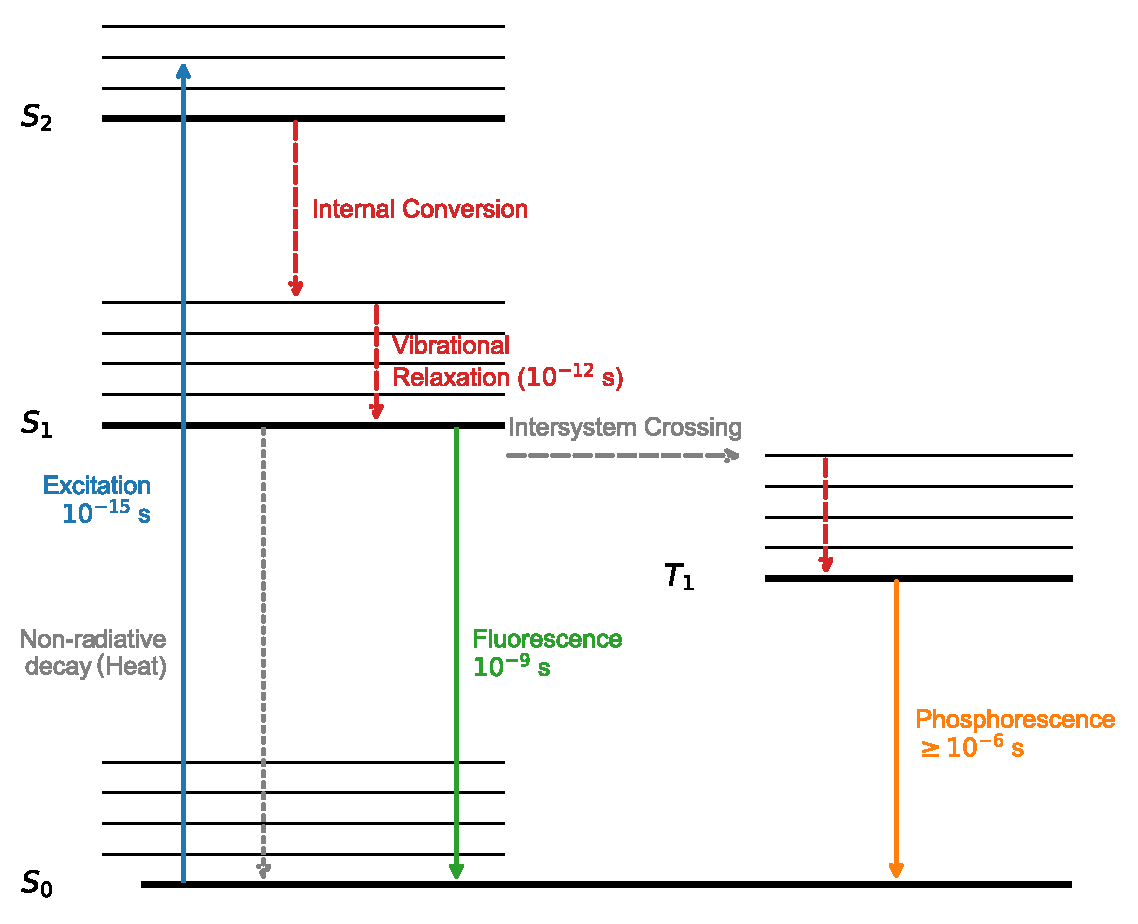
\includegraphics[height = 5cm]{Fig/Fig04.pdf}
    \caption{}
    \label{fig4}
  \end{subfigure}
  \begin{subfigure}[b]{0.45\textwidth}
    \centering
    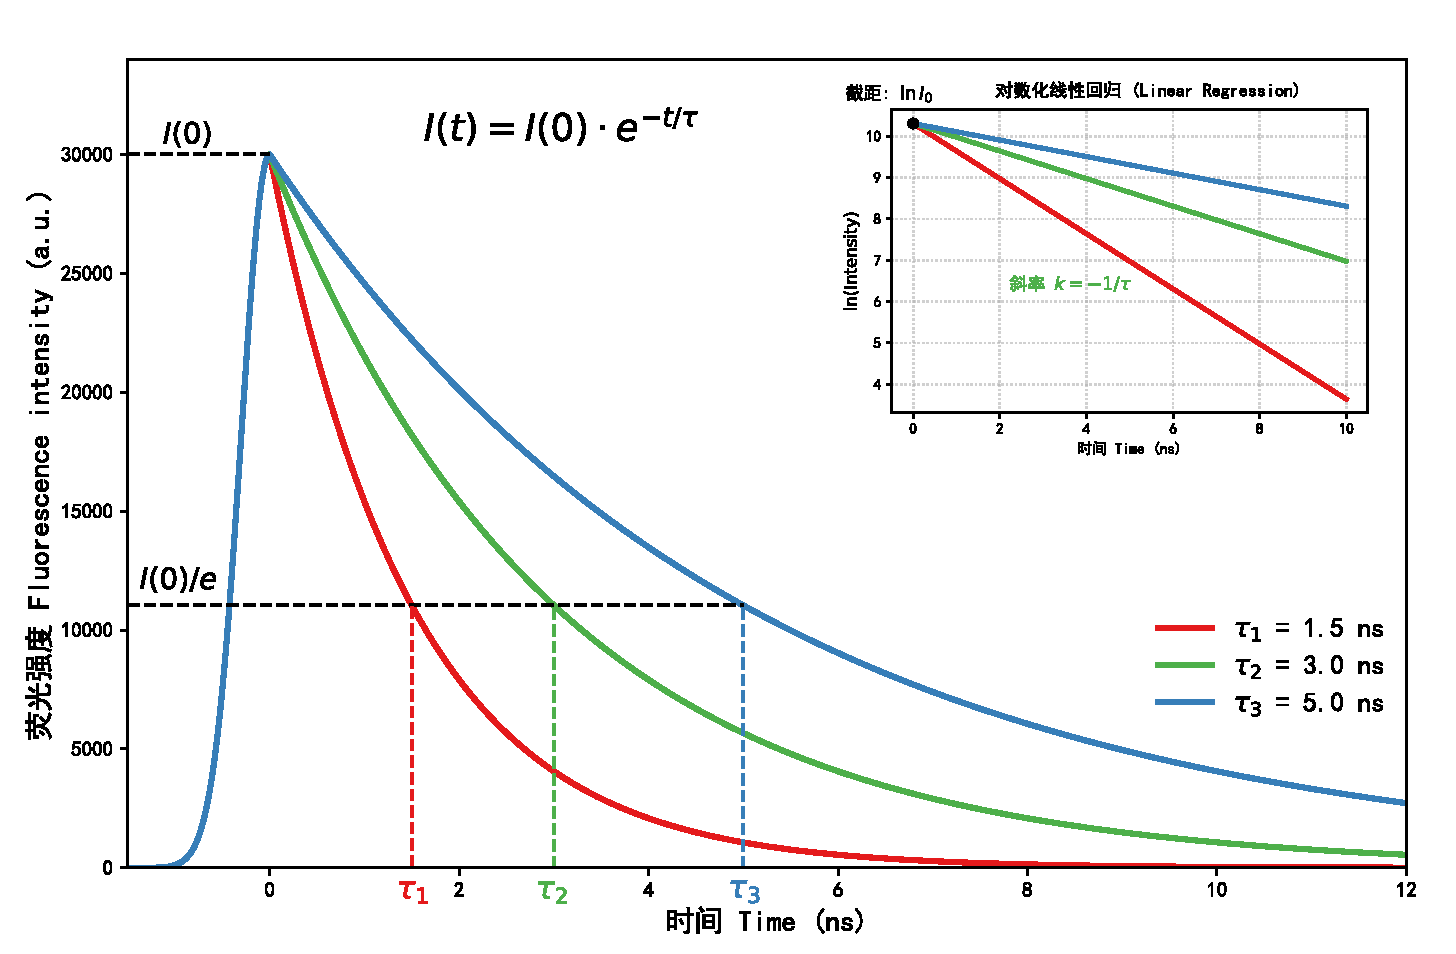
\includegraphics[height = 5cm]{Fig/Fig05.pdf}
    \caption{}
    \label{fig5}
  \end{subfigure}
  \bicaption{荧光寿命的物理机制与单指数衰减表征示意图。(a) Jablonski 能级图示意\cite{RN568}；(b) 单指数荧光衰减及其对数线性拟合示意}{Physical mechanism of fluorescence lifetime and schematic of single-exponential decay characterization. (a) Jablonski diagram\cite{RN568}; (b) single-exponential fluorescence decay and its semi-logarithmic fitting}
  \label{fig4-5}
\end{figure}

根据 Kasha 定律，无论分子最初被激发到哪个更高激发态，其发光过程通常都发生在最低激发单重态 $S_1$ 的最低振动能级。这是因为分子会在皮秒甚至更短时间尺度内，先通过振动弛豫和内部转换迅速回到 $S_1$ 态的最低振动态，随后再发生荧光发射。因此，大多数荧光发射光谱主要由 $S_1 \rightarrow S_0$ 跃迁决定。

除荧光外，分子还可能通过系间窜越(intersystem crossing, ISC)由单重态跃迁至三重态，例如 $S_1 \rightarrow T_1$。由于三重态到基态的跃迁在量子力学上通常是自旋禁阻的，因此三重态寿命通常远长于单重态，对应的磷光发射时间尺度常可达到微秒至秒量级。对于本文关注的 FLIM 而言，主要测量对象仍然是纳秒量级的荧光衰减过程。

在单指数近似下，若激发态分子的辐射跃迁速率常数和非辐射跃迁速率常数分别为 $k_r$ 和 $k_{nr}$，则激发态总失活速率为两者之和，因此荧光寿命可写为:

\begin{equation}
  \tau=\frac{1}{k_r+k_{nr}}
\end{equation}

相应地，荧光量子产率 $\Phi$ 定义为发射荧光光子数与吸收光子数之比，其物理意义是辐射失活在总失活中的占比，因此可表示为:

\begin{equation}
  \Phi=\frac{k_r}{k_r+k_{nr}}
\end{equation}

可以看出，寿命 $\tau$ 与量子产率 $\Phi$ 虽然形式相似，但物理含义不同：前者表征激发态持续时间，后者表征辐射发射效率。若定义辐射寿命 $\tau_r=1/k_r$，则还可进一步写为:

\begin{equation}
  \Phi = k_r\tau=\frac{\tau}{\tau_r}
\end{equation}

因此，当非辐射过程增强时，寿命和量子产率通常都会下降；反之，当体系更倾向于辐射跃迁时，荧光寿命和量子产率则可能同时提高。



\subsection{荧光衰减模型与寿命提取}\label{5.1.2}

\begin{figure}[htbp]
    \centering

    \begin{subfigure}[b]{0.80\textwidth}
        \centering
        \includegraphics[width=\textwidth]{Fig/Fig06-1.pdf}
        \caption{}
        \label{fig06a}
    \end{subfigure}
    \vspace{0.2cm}
    \begin{subfigure}[b]{0.42\textwidth}
        \centering
        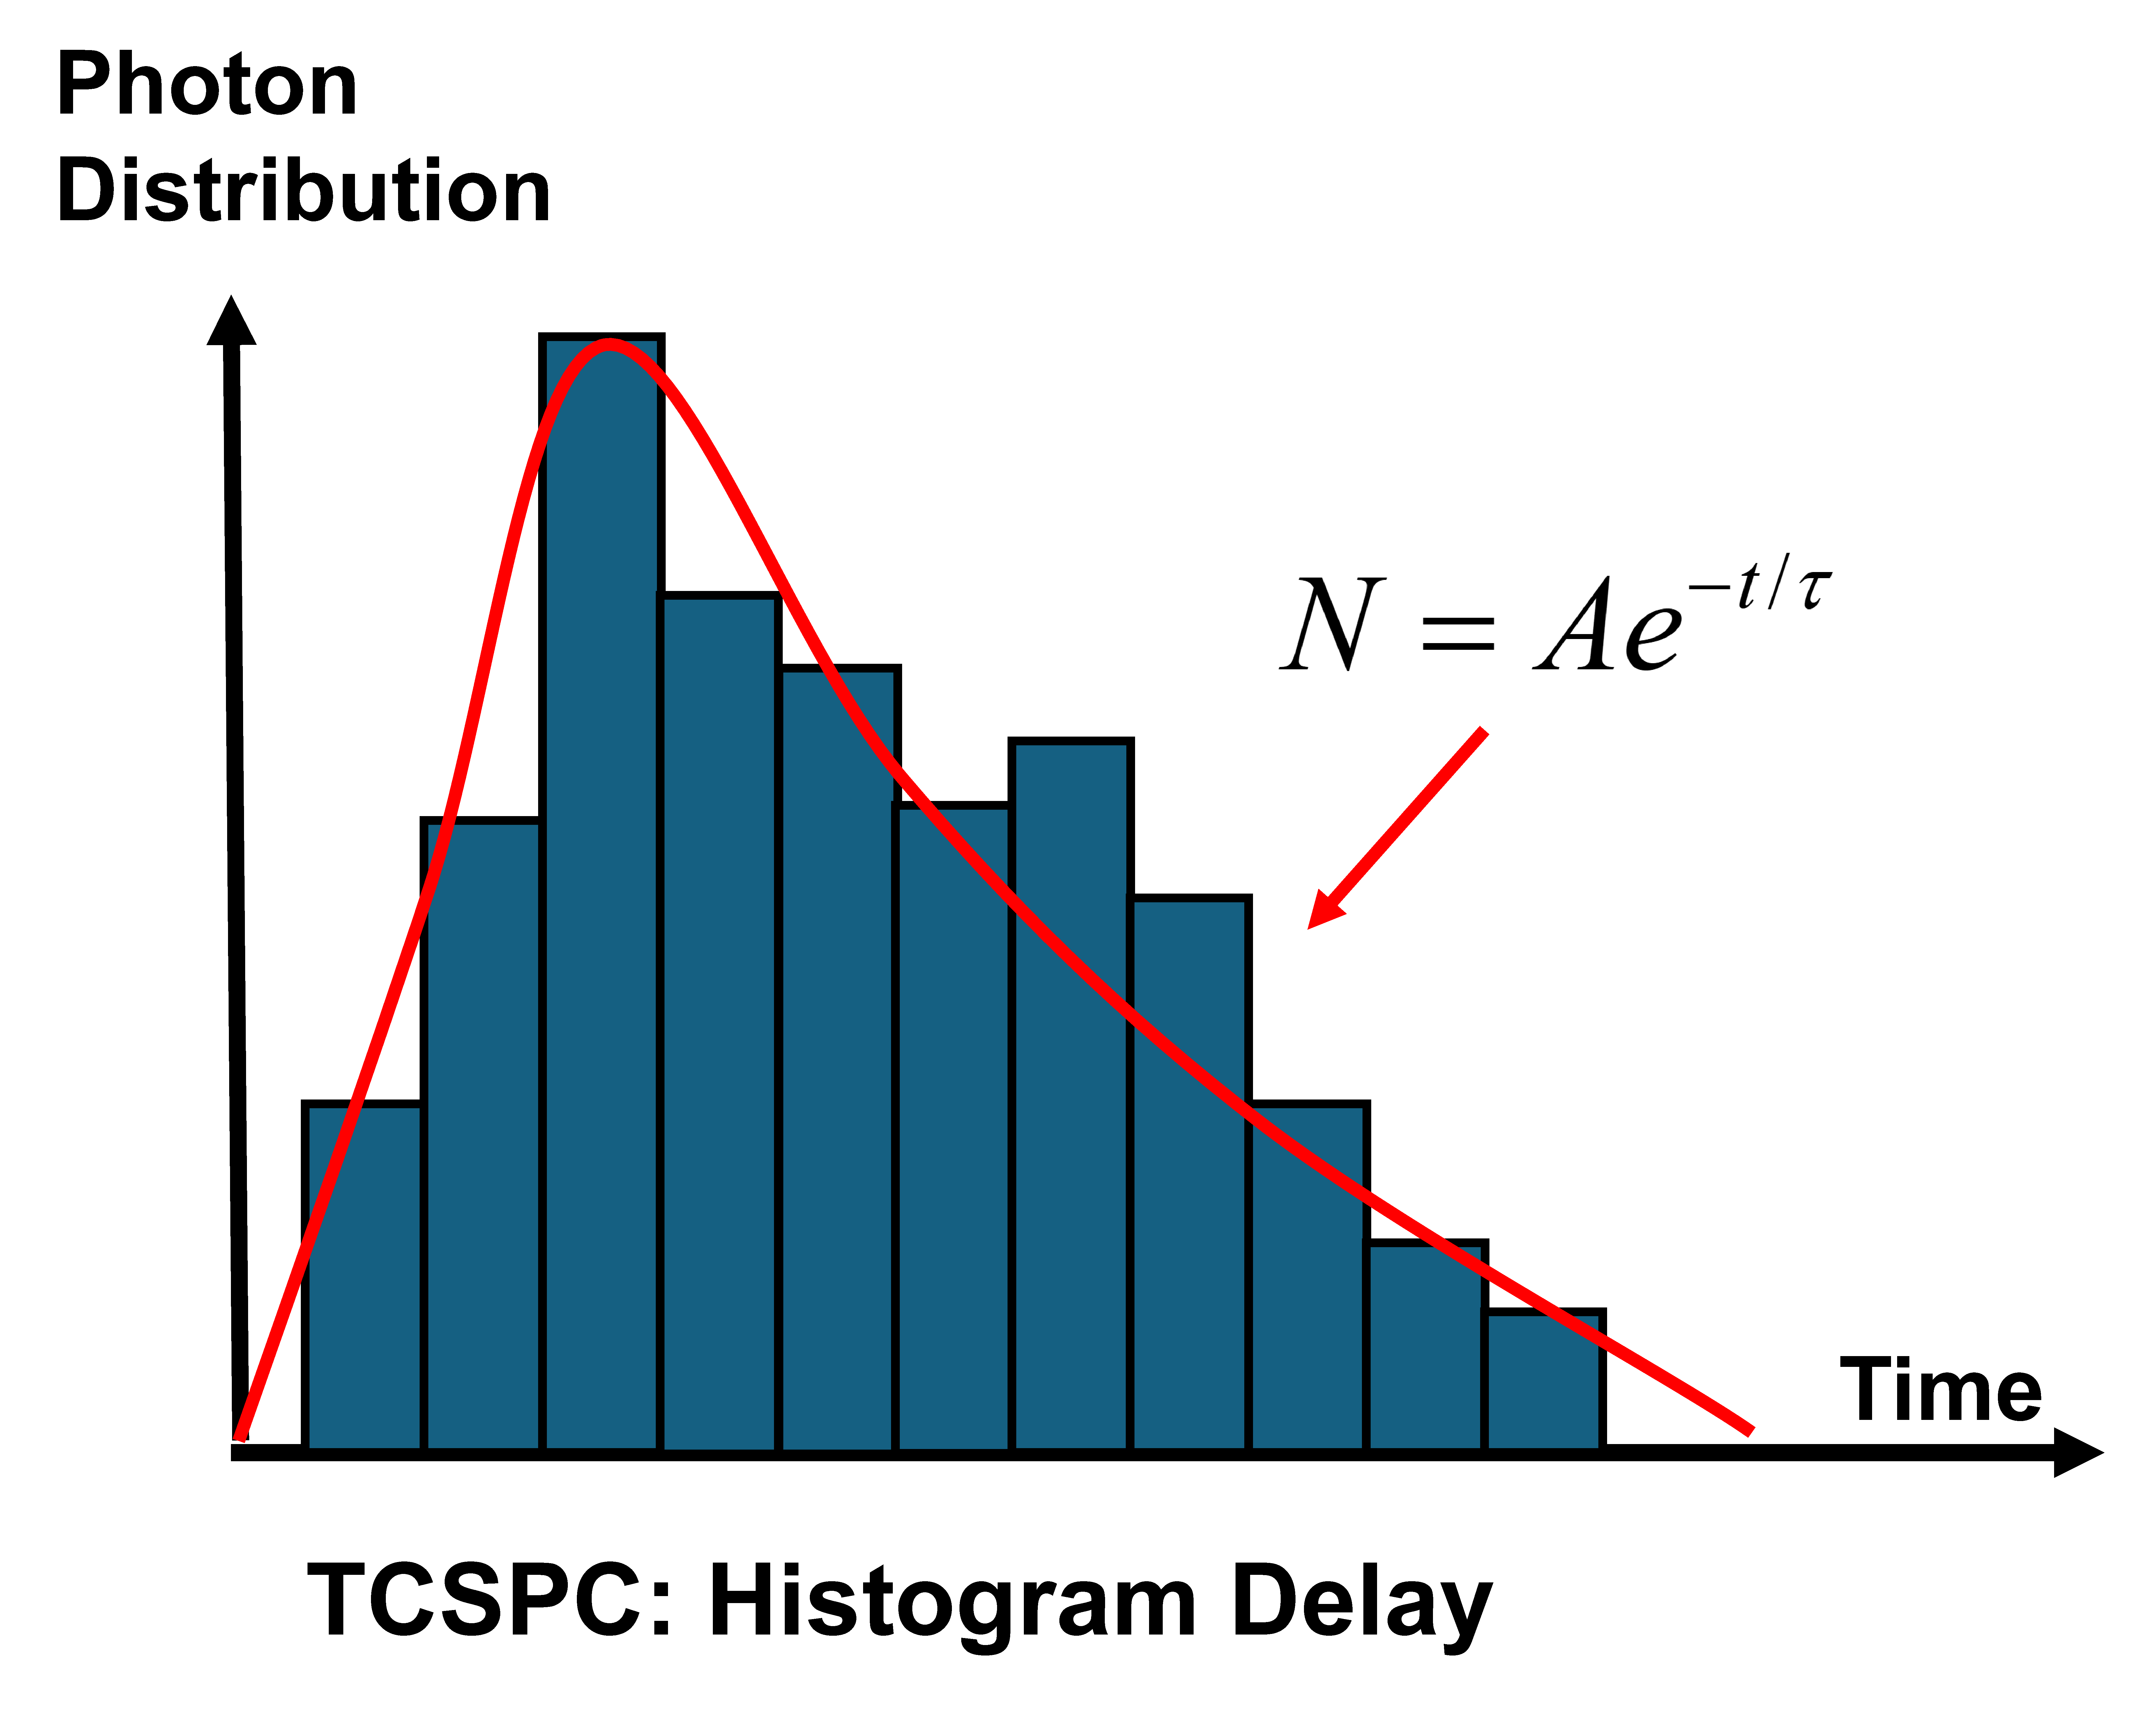
\includegraphics[width=\textwidth]{Fig/Fig06-2.pdf}
        \caption{}
        \label{fig06b}
    \end{subfigure}
    \hfil%
    \begin{subfigure}[b]{0.44\textwidth}
        \centering
        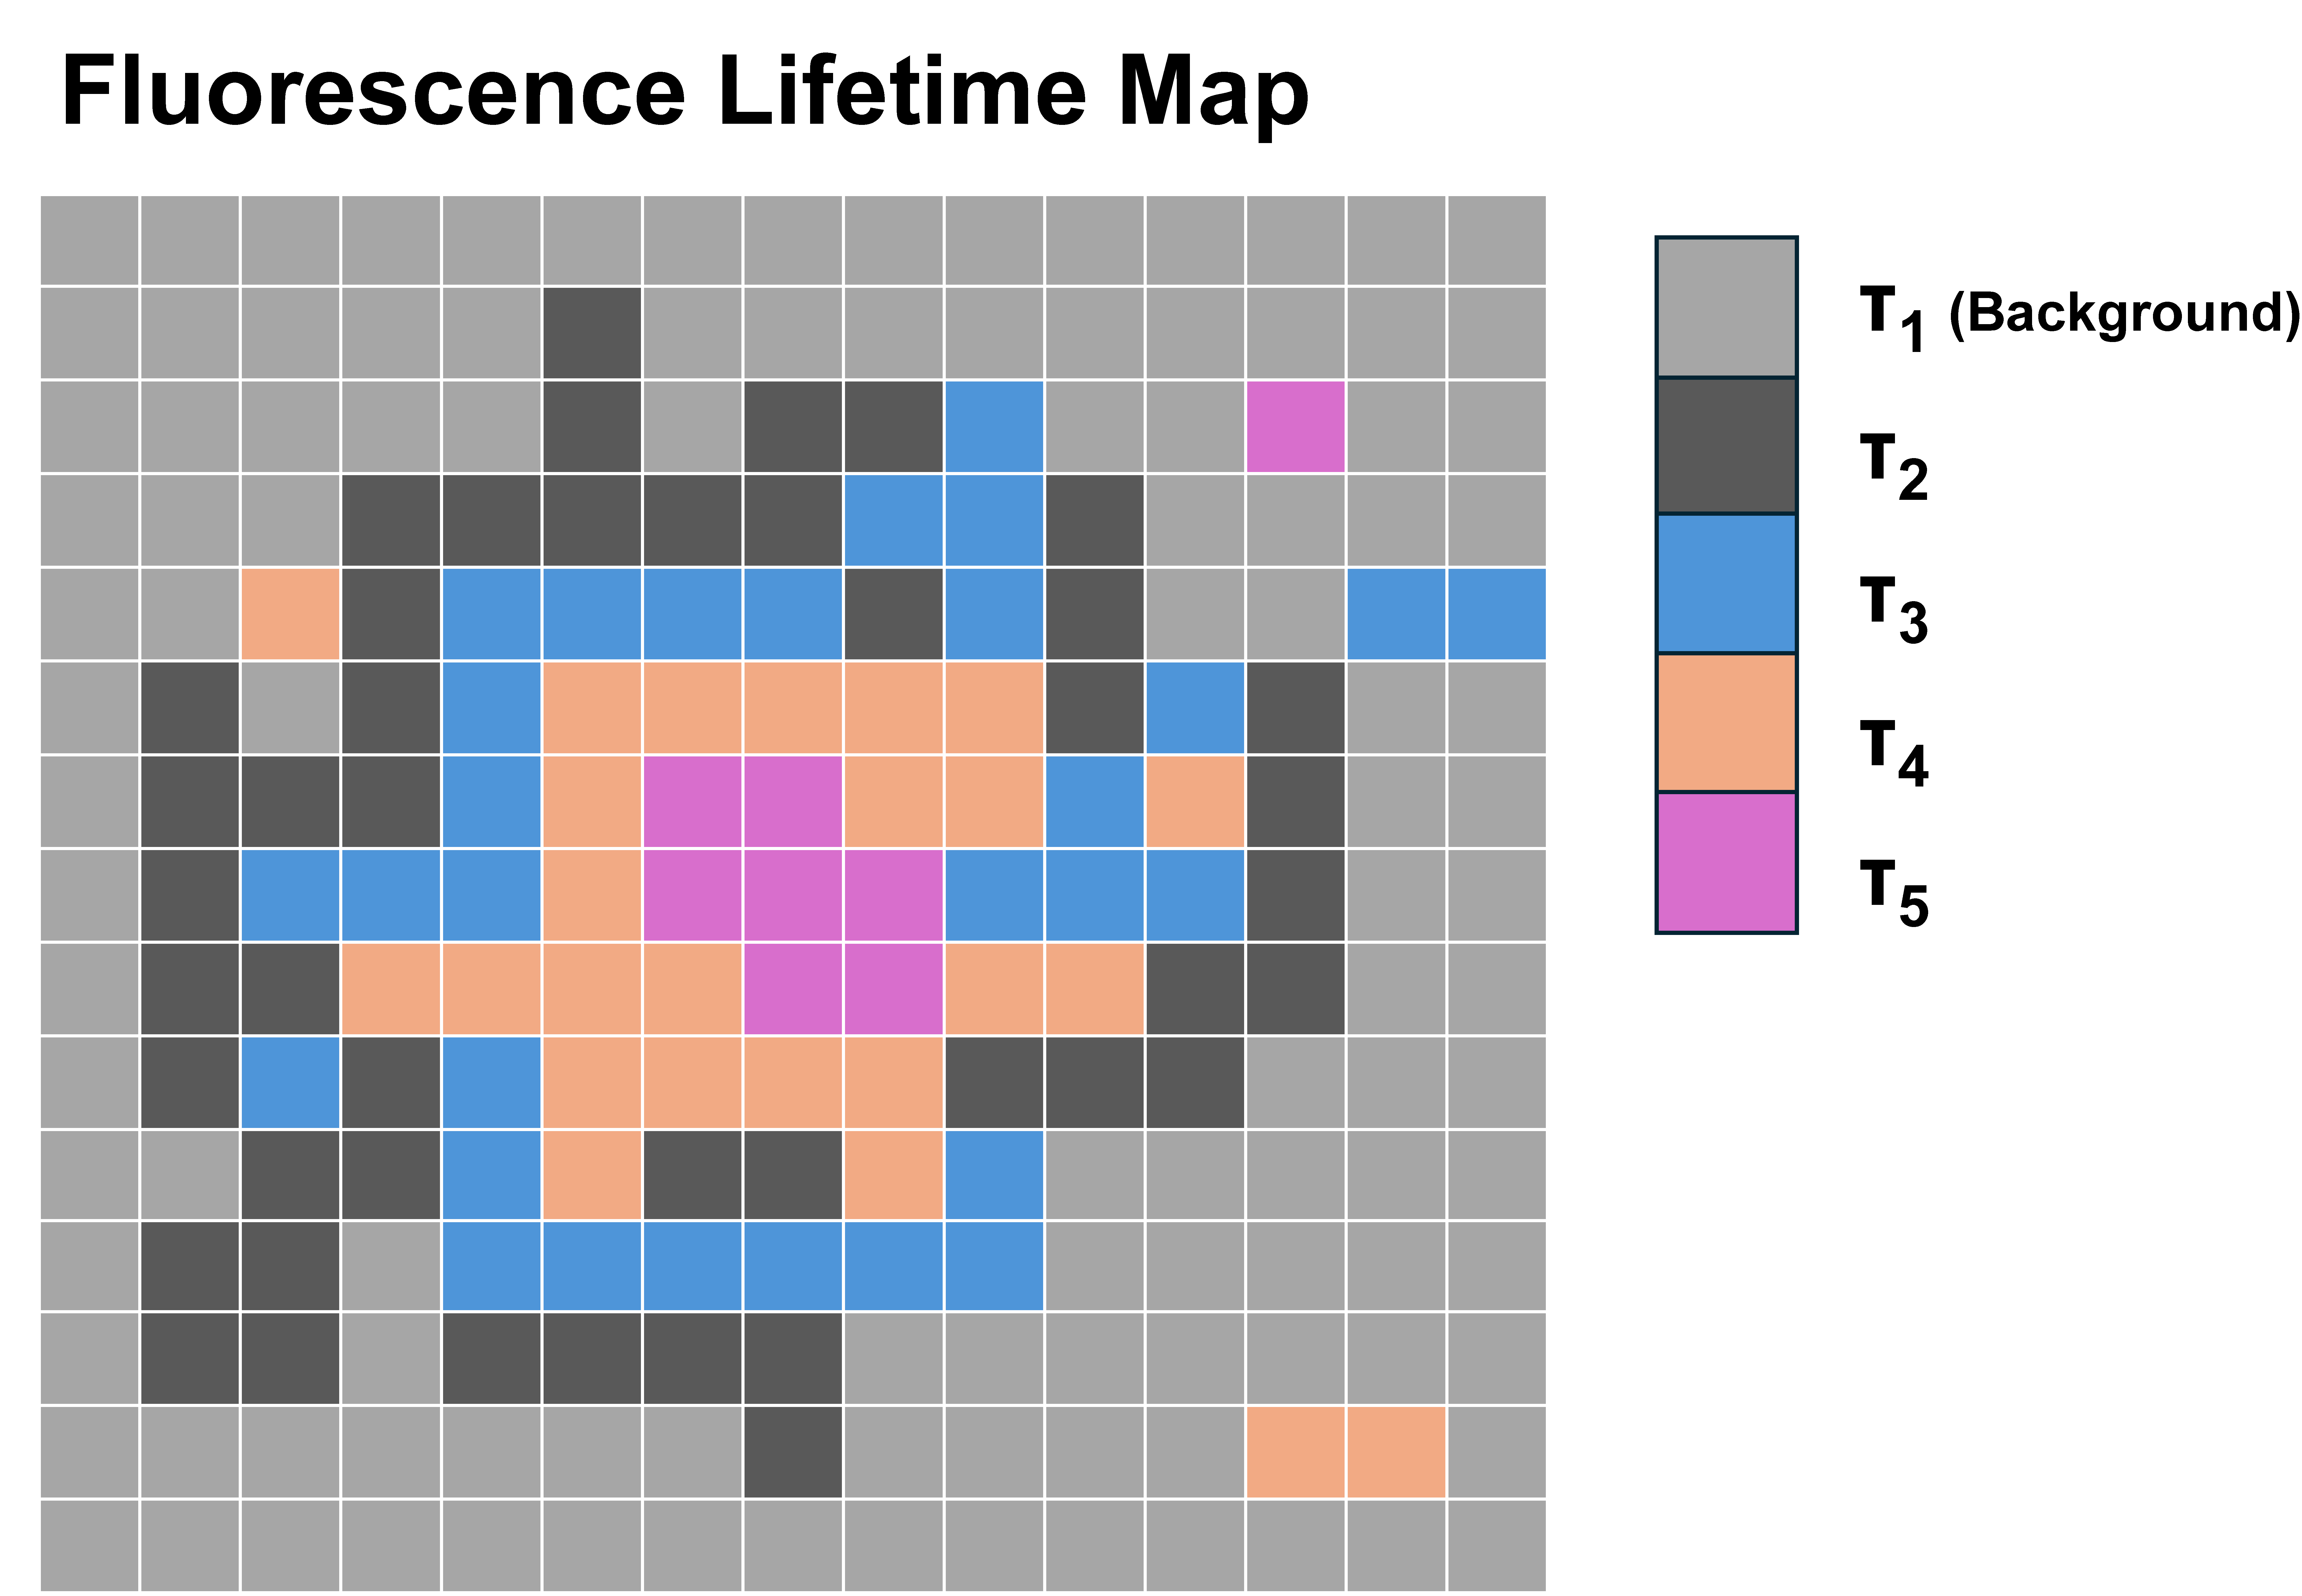
\includegraphics[width=\textwidth]{Fig/Fig06-3.pdf}
        \caption{}
        \label{fig06c}
    \end{subfigure}

    \bicaption{基于 TCSPC 的荧光寿命获取与图像重建示意图。(a) 激发脉冲与荧光发射之间的时间延迟测量原理；(b) 多次光子到达事件累积形成 TCSPC 延迟时间直方图的过程；(c) 基于像素级荧光衰减拟合得到的荧光寿命分布图}
    {Schematic of fluorescence-lifetime acquisition and image reconstruction based on TCSPC. (a) Principle of measuring the temporal delay between excitation pulses and fluorescence emission; (b) formation of the TCSPC histogram through accumulation of photon arrival events; (c) fluorescence lifetime map reconstructed from pixel-wise fitting of fluorescence decay curves}
    \label{fig06}
\end{figure}


若有 $N(t)$ 个分子处于激发态，则在时间间隔 $dt$ 内，其失活动力学满足:

\begin{equation}
  \frac{dN(t)}{dt}=-(k_r+k_{nr})N(t)
\end{equation}

求解该微分方程可得:

\begin{equation}
  N(t)=N_0 e^{-t/\tau}
\end{equation}

其中 $\tau=1/(k_r+k_{nr})$。由于荧光发射强度与激发态粒子数成正比，因此单指数衰减模型下的荧光强度可表示为:

\begin{equation}
  I(t)=I_0 e^{-t/\tau}
\end{equation}

对于单指数衰减，测得的寿命参数 $\tau$ 与激发态平均寿命在数值上相等。然而，在实际生物样品中，由于荧光分子所处微环境、结合状态或局部淬灭条件往往不均一，荧光衰减常呈现多指数行为，可写为:

\begin{equation}
  I(t)=\sum_i A_i e^{-t/\tau_i}
\end{equation}

其中 $\tau_i$ 表示不同衰减组分的寿命，$A_i$ 为对应振幅。对于多指数衰减，常可根据具体应用定义振幅加权平均寿命或强度加权平均寿命，以表征整体衰减过程。

图~\ref{fig06} 示意了 FLIM 数据从光子探测到寿命图像重建的基本过程。首先，样品中的荧光分子在脉冲激光激发下吸收光子并产生荧光发射；随后，系统采用 TCSPC 方法对到达探测器的荧光光子进行时间统计，并在每个像素位置建立对应的荧光衰减直方图。通过对该衰减曲线进行寿命拟合，可获得该像素对应的寿命参数 $\tau$。最终，将逐像素拟合得到的寿命值重新映射到空间坐标中，即可形成荧光寿命图像。图中不同颜色代表不同的荧光寿命，从而反映样品内部不同微环境或不同分子状态的空间分布。

如图\ref{fig4-5}(\subref{fig5})右上角子图部分，在单指数近似下，对衰减曲线取自然对数可得到:

\begin{equation}
  \ln I(t)=\ln I_0-\frac{t}{\tau}
\end{equation}

因此，$\ln I(t)$ 与时间 $t$ 之间呈线性关系，其斜率为 $-1/\tau$，截距为 $\ln I_0$。图~\ref{fig4-5}(\subref{fig5}) 给出了单指数荧光衰减及其对数线性拟合示意。需要指出的是，这种对数线性回归方法适用于信噪比较高、且衰减行为近似单指数的初步估计；对于实际 TCSPC 数据，通常还需要结合仪器响应函数进行卷积拟合，以获得更准确的寿命结果。




\section{仪器响应函数(IRF)标定与同步延迟校准}\label{5.2}

在 FLIM 系统中，仪器响应函数(instrument response function, IRF)用于表征探测链路与 TCSPC 计时电子学共同引入的时间展宽，是寿命拟合与反卷积分析的基础参数。理想情况下，若输入信号为近似瞬时脉冲，则系统输出的时间响应即为 IRF。实际实验中，通常采用尿素晶体等样品产生的二次谐波(second harmonic generation, SHG)信号作为近似瞬时响应，以测定系统 IRF。

除 IRF 标定外，还需校准同步参考信号与荧光探测信号之间的相对时序\cite{RN94}。由于电信号在电缆中的传播速度低于真空光速，因此不同长度的同轴电缆会引入固定的传播延迟，其延迟可表示为:

\begin{equation}
  t_d=\frac{L}{v}=\frac{L}{VF\cdot c}
\end{equation}

其中 $L$ 为电缆长度，$v$ 为电信号在电缆中的相速度，$VF$ 为速度因子(velocity factor)，$c$ 为真空光速。对于常见聚乙烯介质同轴电缆，通常有 $VF\approx 0.66$，因此传播延迟近似为:

\begin{equation}
  t_d \approx 5.0~\text{ns/m}\;(\approx 1.5~\text{ns/ft})
\end{equation}

若电缆长度变化为 $\Delta L$，则其引入的时间偏移满足:

\begin{equation}
  \Delta t \approx \frac{\Delta L}{VF\cdot c}\approx 5.0~\text{ps/mm}\cdot \Delta L
\end{equation}

该延迟会改变荧光衰减曲线在 TCSPC 时间采样窗口中的位置，从而影响寿命拟合的稳定性与准确性。因此，需要结合标准寿命样品对同步时序进行校准，通过调整同步电缆长度，或等效地修改 TCSPC 的时间零点与同步偏置参数，使衰减曲线落在合适的采样窗口内，并获得与标准值一致的拟合寿命。

从系统实现角度看，IRF 标定与同步延迟校准分别对应两类不同问题：前者解决的是``系统本身会将一个理想瞬时信号展宽到什么程度''，后者解决的是``参考时钟与探测信号在时间轴上是否正确对齐''。只有同时完成这两类校准，后续寿命拟合结果才具有可比性和可靠性。

% 如果你后面有 IRF / 时序图，可以加在这里
% \begin{figure}[htbp]
%   \centering
%   \includegraphics[width=0.75\textwidth]{Fig/XXX.pdf}
%   \caption{IRF 测量与同步延迟校准示意图。}
%   \label{fig:irf_sync}
% \end{figure}




\section{FLIM 数据采集与同步模式设计}\label{5.3}

在点扫描 FLIM 系统中，寿命信息的获取不仅依赖于探测器和 TCSPC 电子学本身，还依赖于扫描时序与采集时序之间的严格对应关系。与宽场相机直接输出二维图像不同，点扫描系统中的每一个像素都对应一段时间窗内的光子统计结果，因此必须通过同步信号将``光子到达时间''与``当前扫描位置''正确关联，才能最终重建出荧光寿命图像。也正因为如此，数据采集方式和同步模式的设计，直接决定了 FLIM 图像重建的效率、精度与适用场景。



\subsection{点扫描系统中的时序同步关系}\label{5.3.1}

在点扫描显微镜中，图像采集通常遵循像素(pixel)、行(line)和帧(frame)三级扫描时序。对于一幅 $N\times M$ 像素的扫描图像，系统在完成一个像素的积分后，依次切换至下一像素；当一行中的 $N$ 个像素全部扫描完毕后，产生一次行同步信号(line sync)；当全部 $M$ 行扫描结束后，则产生一次帧同步信号(frame sync)。因此，像素同步信号、行同步信号和帧同步信号共同构成了点扫描 FLIM 图像重建的基本时序框架。

\begin{figure}[htbp]
  \centering
  \begin{subfigure}[b]{0.47\textwidth}
    \centering
    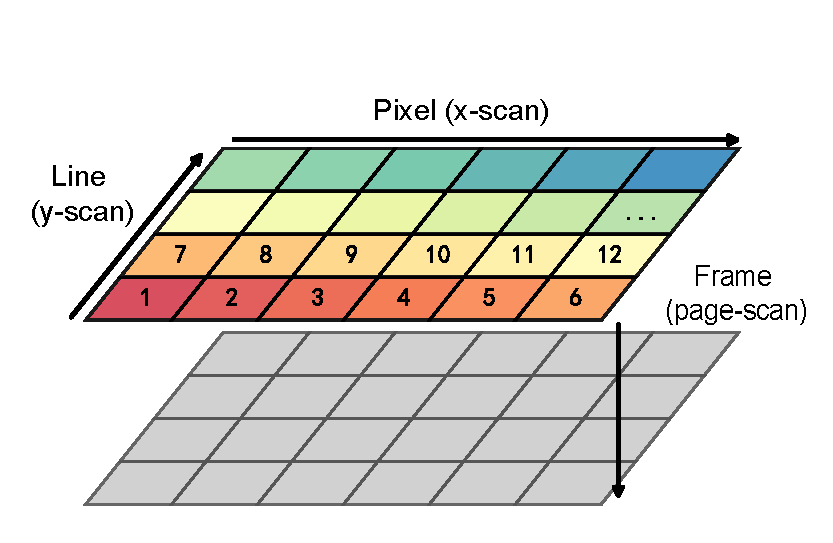
\includegraphics[width=\textwidth]{Fig/Fig18-1.pdf}
    \caption{}
    \label{fig18a}
  \end{subfigure}
  \hfill
  \begin{subfigure}[b]{0.47\textwidth}
    \centering
    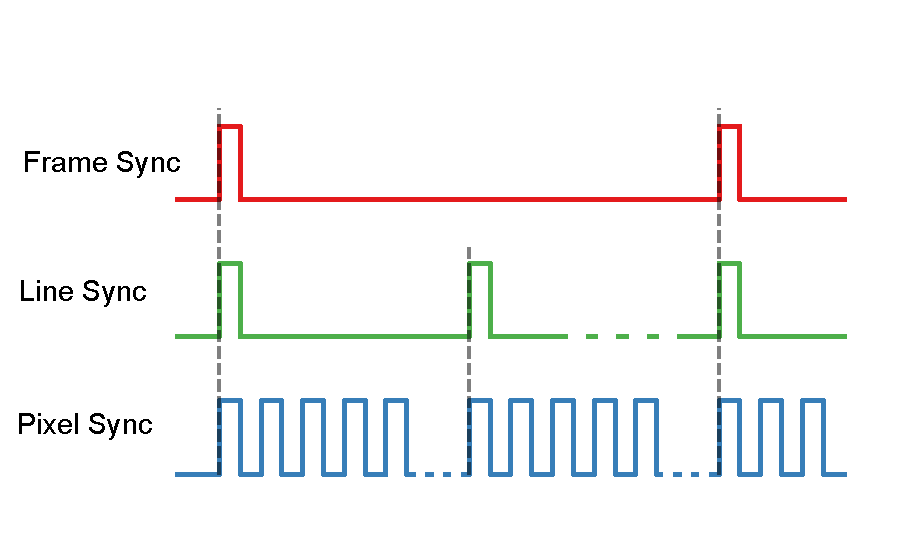
\includegraphics[width=\textwidth]{Fig/Fig18-2.pdf}
    \caption{}
    \label{fig18b}
  \end{subfigure}
  \bicaption{点扫描图像重建中的空间扫描层级与同步时序关系示意。(a) 点扫描图像的像素、行与帧层级关系；(b) 与图像重建对应的 pixel sync、 line sync 和 frame sync 时序关系}
  {Schematic of spatial scanning hierarchy and synchronization timing in point-scanning image reconstruction. (a) Hierarchical organization of pixel, line and frame in point-scanning imaging; (b) timing relationship among pixel sync, line sync and frame sync for image reconstruction}
  \label{fig18}
\end{figure}

图~\ref{fig18}(\subref{fig18a}) 展示了点扫描图像的空间组织方式。在点扫描显微镜中，图像并非一次性并行获取，而是按照像素、行和帧三个层级逐步完成扫描：像素构成单行，若干行构成一帧，因此图像重建本质上依赖于明确的扫描层级与顺序信息。

图~\ref{fig18}(\subref{fig18b}) 则进一步给出了与上述空间扫描过程相对应的多级同步信号关系。pixel sync 用于标记像素采样或积分节拍，line sync 用于标记每一行的起止与切换，frame sync 则用于标记整帧的开始或结束。只有将光子事件的到达时间与这三级同步信号正确关联，TCSPC 记录得到的时间信息才能被准确映射回图像中的空间位置，最终完成荧光寿命图像的重建。

在此基础上，本文采用了两类不同的 FLIM 数据采集模式：一类是单路同步采集模式，另一类是三路同步采集模式。两种方式各有特点，分别适用于不同的成像任务与硬件条件。

在实际系统中，不同硬件平台对上述三级同步信息的接入方式并不完全一致。根据采集卡可接收同步信号通道数、数据缓存方式以及后端重建策略的不同，本文进一步采用了单路同步采集和三路同步采集两种实现模式。


\subsection{单路同步采集模式}\label{5.3.2}

单路同步模式可视为一种逐像素寿命获取策略。在该模式下，系统仅使用一路触发信号控制寿命数据的采集与保存，即当触发信号到来时，采集卡开始对当前扫描位置对应的荧光时间信息进行记录。每个像素点的寿命数据被单独保存，随后再结合扫描顺序或像素坐标信息，将这些独立数据重新映射为完整的二维寿命图像。

这种方式的优点在于控制结构相对简单，易于在自研硬件和非标准扫描流程下实现，并且对不规则扫描区域或自定义 ROI 成像具有较高灵活性。对于需要逐点分析、逐点存储或特殊扫描路径控制的实验任务，单路同步模式具有较强适配性。

特别是对于一些基础的商用采集卡如我们使用的SA230P(Acqiris)，通常只有一个外部采集触发端口，这时使用单路同步进行采集触发并后续进行像素分配更合适。实验室自研的采集卡中同样有这样的问题，当外部触发过多容易产生时序干扰，因此我们同样选定单路同步模式对于自研采集卡的使用。

\begin{figure}[htbp]
  \centering
  \begin{subfigure}[b]{0.42\textwidth}
    \centering
    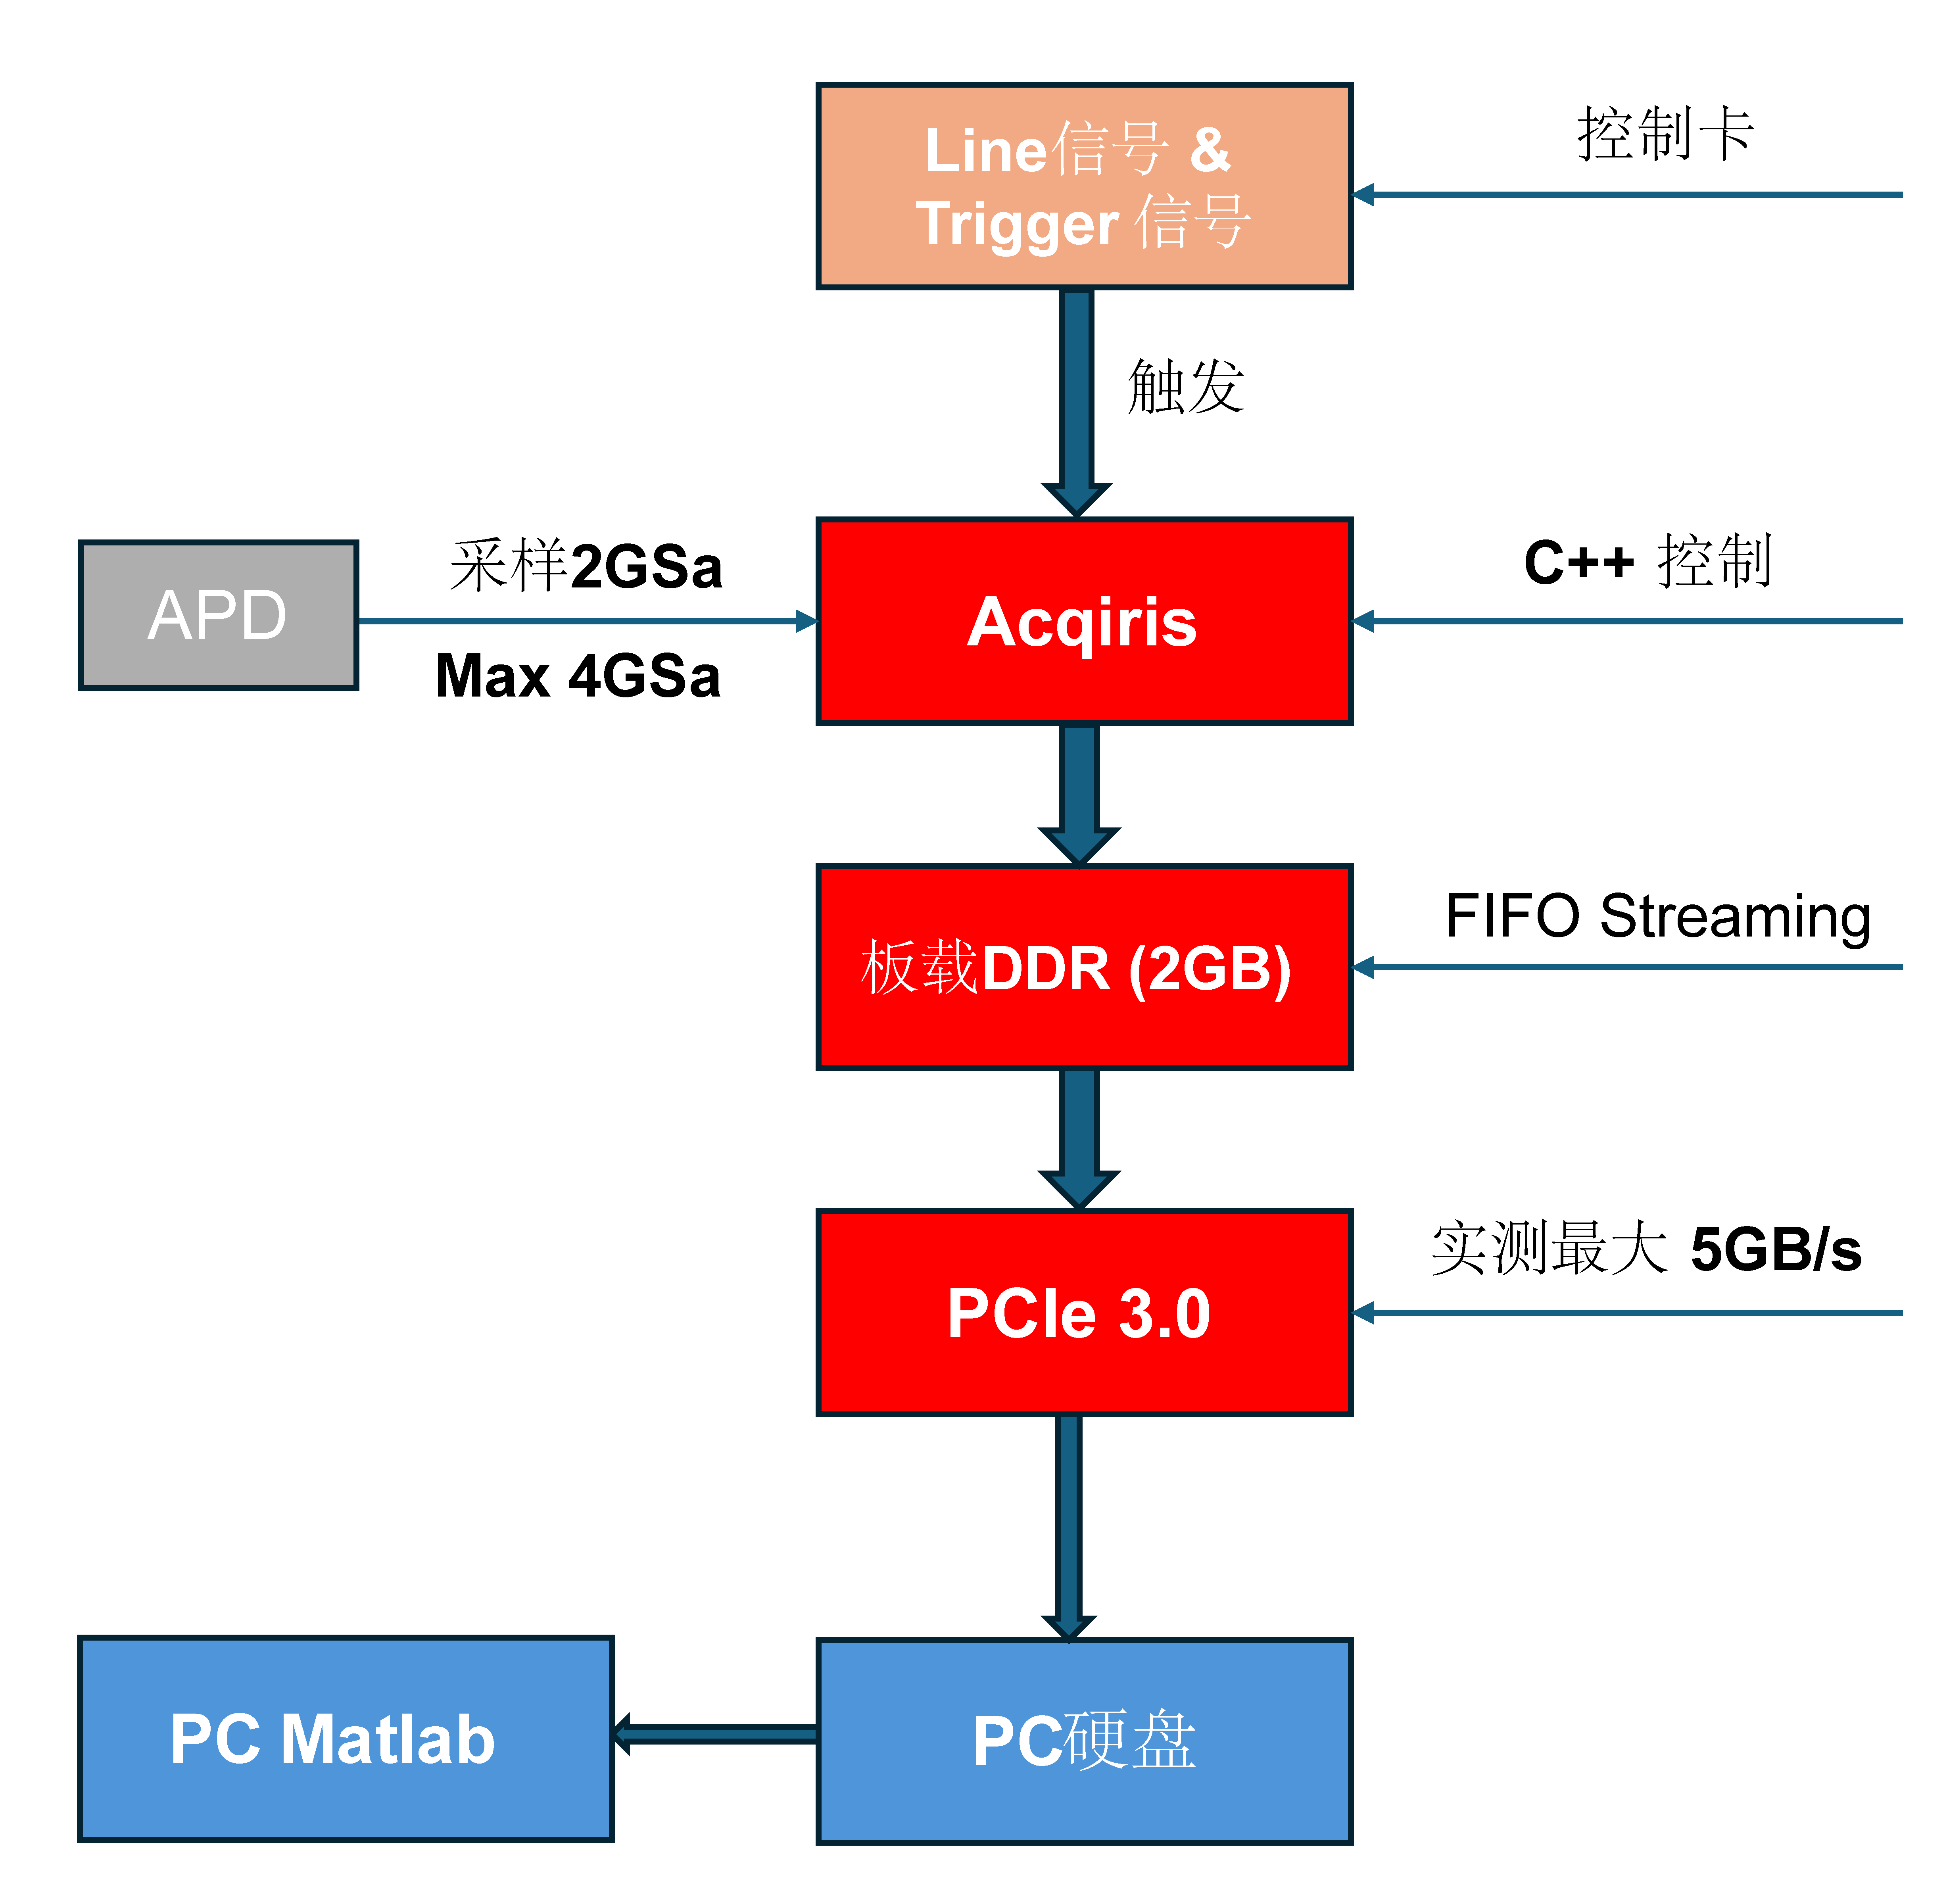
\includegraphics[width = \textwidth]{Fig/Fig19.pdf}
    \caption{}
    \label{fig19}
  \end{subfigure}
  \hfill
  \begin{subfigure}[b]{0.56\textwidth}
    \centering
    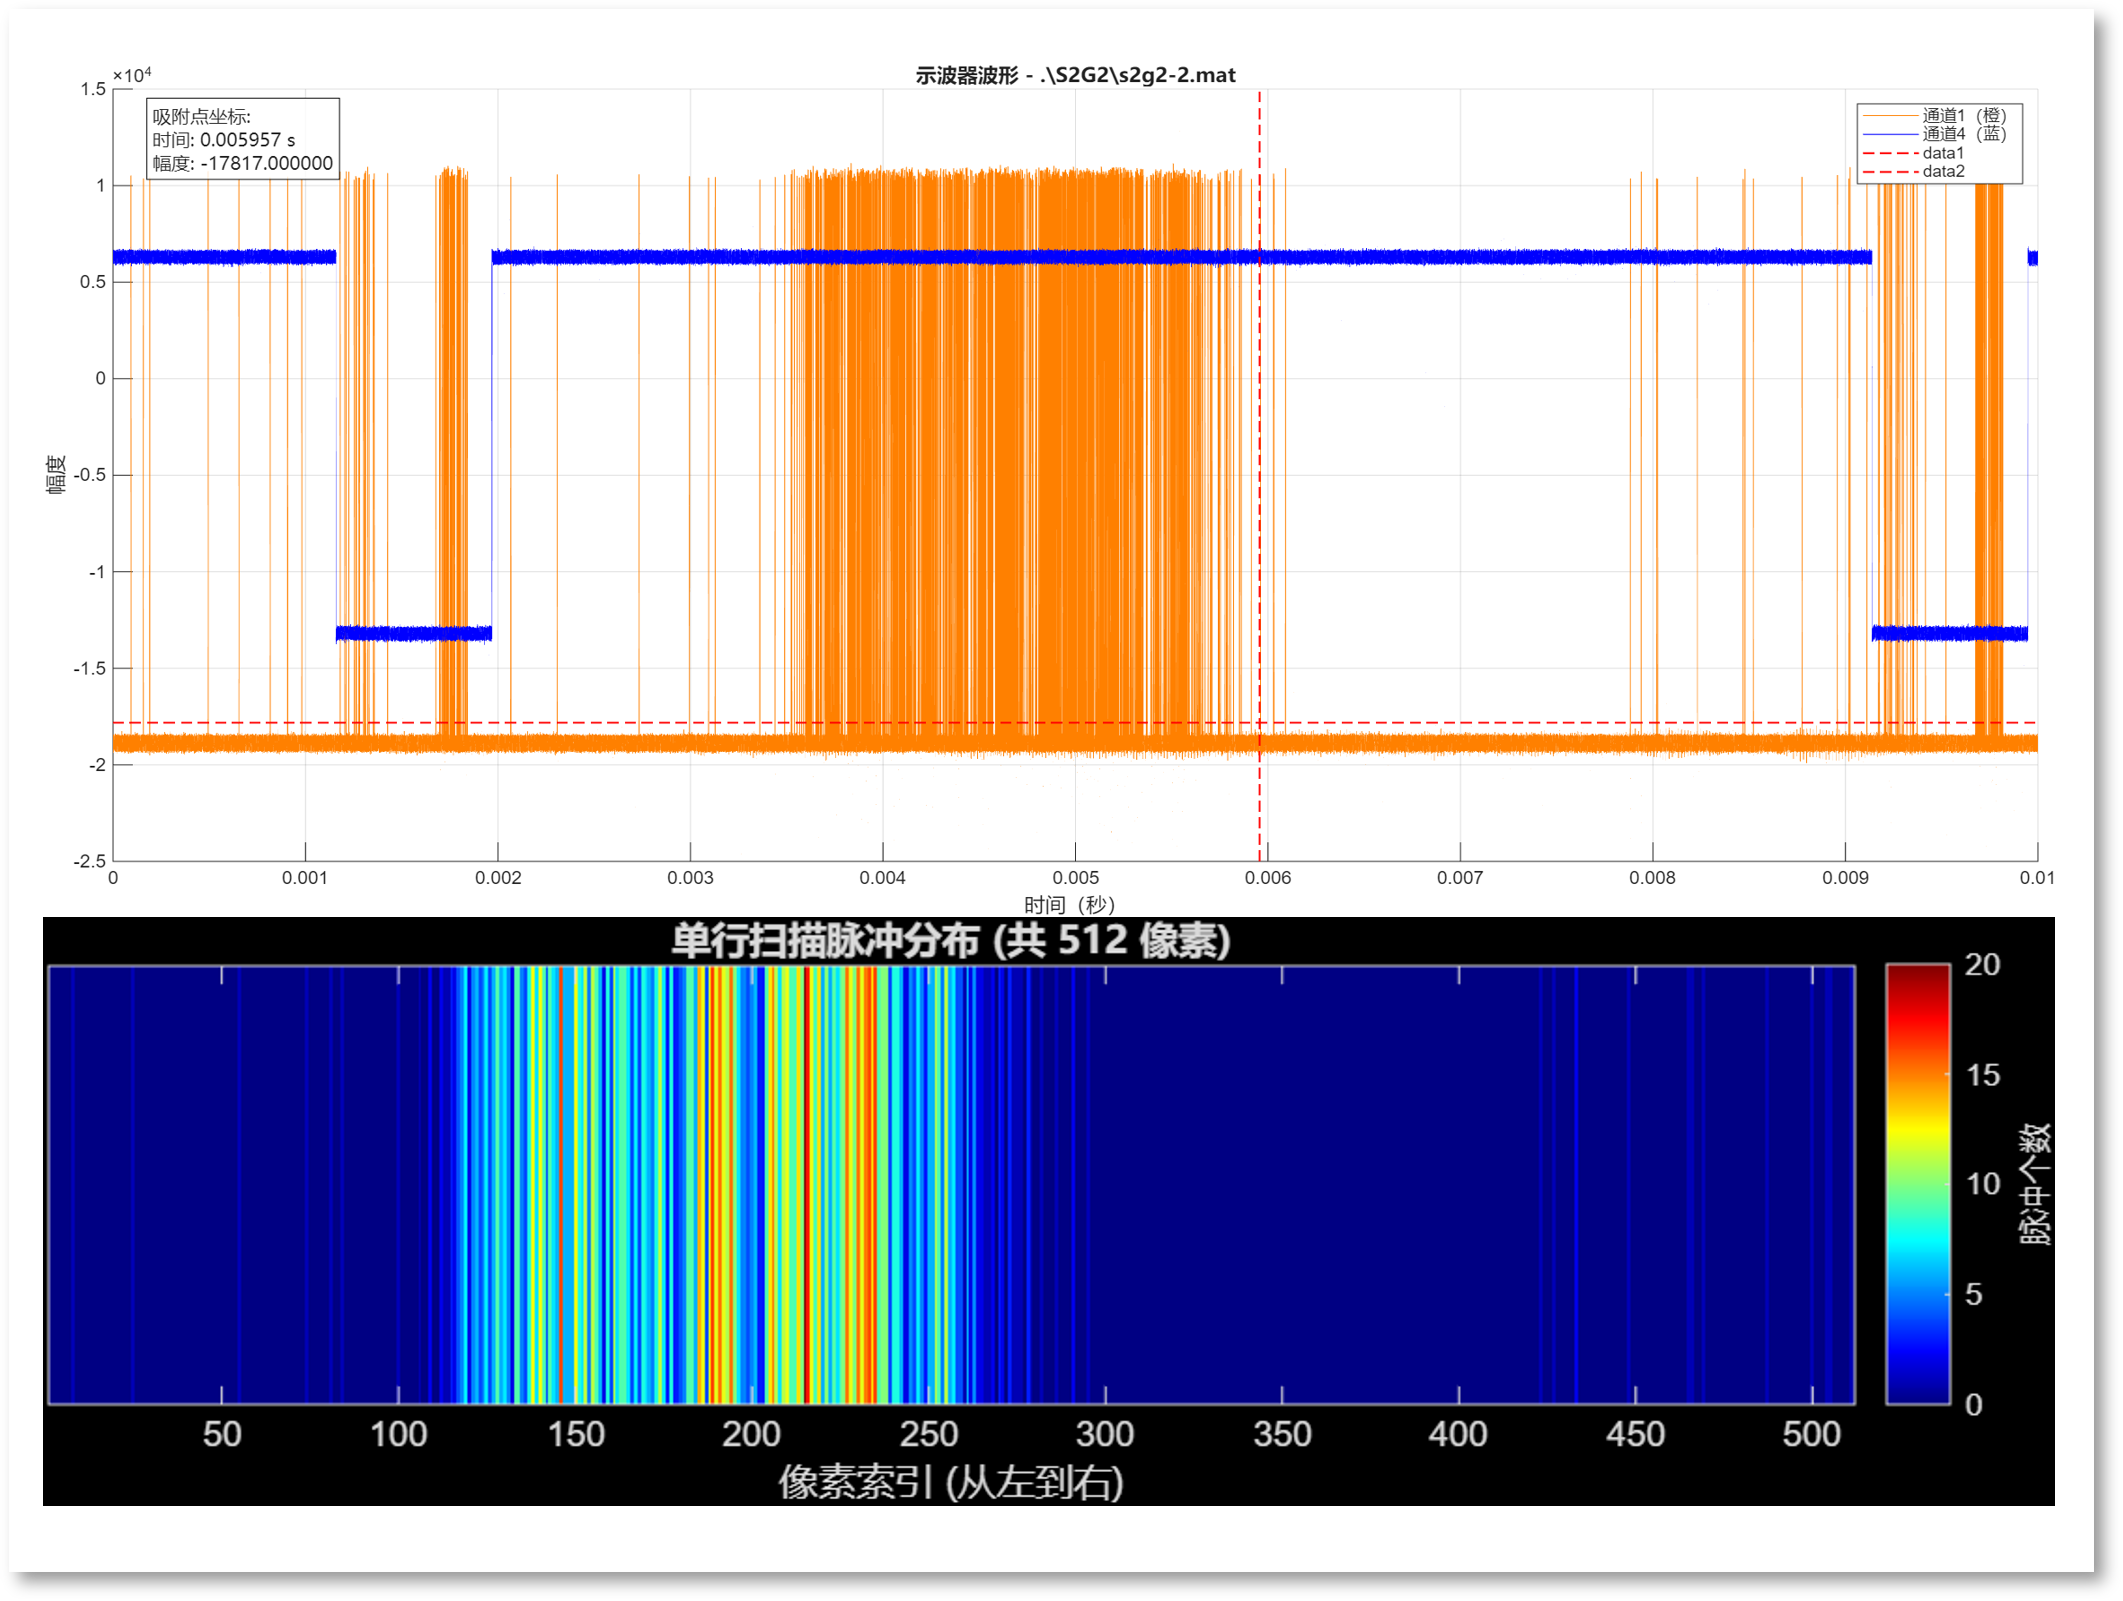
\includegraphics[width = \textwidth]{Fig/Fig20.png}
    \caption{}
    \label{fig20}
  \end{subfigure}
  \bicaption{单路同步采集模式中的数据流与采样分布示意。(a) 单路同步模式下的数据采集流程；(b) 单路同步下某一行信号的光子分布密度}{Data flow and sampling distribution in the single-channel synchronized acquisition mode. (a) Data-acquisition flow in the single-channel synchronized mode; (b) photon-density distribution along one scanned line}
  \label{fig19-20}
\end{figure}

图~\ref{fig19-20}(\subref{fig19}) 展示了单路同步模式下的数据采集流程。除 CPU 端部分处理可并行执行外，数据触发、读取、保存与重分配等关键环节大多需要顺序进行，因此系统总体采集带宽通常受限于链路中最慢的环节，表现出典型的``木桶效应''。这意味着单路同步模式虽然实现简单，但在高数据量场景下容易受到存储与数据吞吐带宽的限制。

图~\ref{fig19-20}(\subref{fig20}) 则给出了单路同步模式下一行扫描数据的示波器观测结果及其数字化重分配示意。蓝色通道表示 line 信号的起止，橙色信号表示对应荧光响应；下方则示意将该行数据重分配到 512 个像素后的信号密度分布。




\subsection{三路同步采集模式}\label{5.3.3}

与单路同步不同，三路同步模式同时引入像素、行和帧三类同步信号，用于协调寿命信息的采集、缓存与写入过程。该模式通常依赖 TCSPC 板卡内部的 FIFO 缓冲与图像文件预分配机制：系统首先预先建立与扫描图像格式对应的寿命图像文件，随后 TCSPC 记录到的光子数据在 pixel、line 和 frame 三类同步信号的共同控制下，按照既定顺序直接写入相应像素位置，从而实现扫描过程与寿命图像生成过程的同步进行。

相较于单路同步模式，三路同步模式的最大优点在于成像效率更高。由于系统能够直接利用多级同步信号完成寿命数据与扫描坐标的对应关系建立，因此在规则矩形区域的栅格扫描中，可直接生成寿命图像，而无需在后处理阶段再进行复杂的逐像素重构或者像素分配。


但与此同时，三路同步模式对扫描方式的规则性要求更高。当成像区域不是标准矩形，或者各扫描行对应的像素数不一致时，数据组织和图像重建会变得更加复杂，从而降低该模式对不规则 ROI 成像的灵活性。因此，三路同步模式更适合规则区域的高速成像，而单路同步模式则更适合灵活路径扫描和特殊实验设计。

图~\ref{fig21-22}(\subref{fig21}) 给出了基于三路同步模式获得的 FLIM 图像结果及其与系统功率的关系。上方图像中，左图为反射式共聚焦成像结果，右图为利用 line、frame 和 sync 三路信号触发 TCSPC 板卡后获得的荧光寿命图像。两者在空间位置上能够良好重叠，说明三路时序同步关系建立正确，系统能够将寿命信息准确映射到对应的扫描位置。

图~\ref{fig21-22}(\subref{fig22}) 下方图像则给出了不同激发功率条件下的 TCSPC 成像结果。可以看出，随着激发功率增加，探测到的荧光信号增强，寿命图像亮度提高；但当功率过高时，系统可能出现局部计数过高、光子堆积和图像过曝等现象，从而影响寿命拟合的准确性。

需要指出的是，单路同步与三路同步的差异主要体现在同步信号组织方式、硬件接口要求以及后处理流程复杂度上，而不体现在寿命拟合模型本身。对于相同的扫描参数、光子统计条件和拟合方法，两种模式在寿命拟合精度及拟合速度上无本质差别。本文建立单路同步采集链路的主要目的，在于针对仅具备单触发输入的采集硬件（如 Acqiris SA230P 采集卡及自研采集卡）提供一种可行的 FLIM 实现路径，从而扩展系统在不同硬件条件下的适用性。


\begin{figure}[htbp]
  \centering
  \begin{subfigure}[b]{0.7\textwidth}
    \centering
    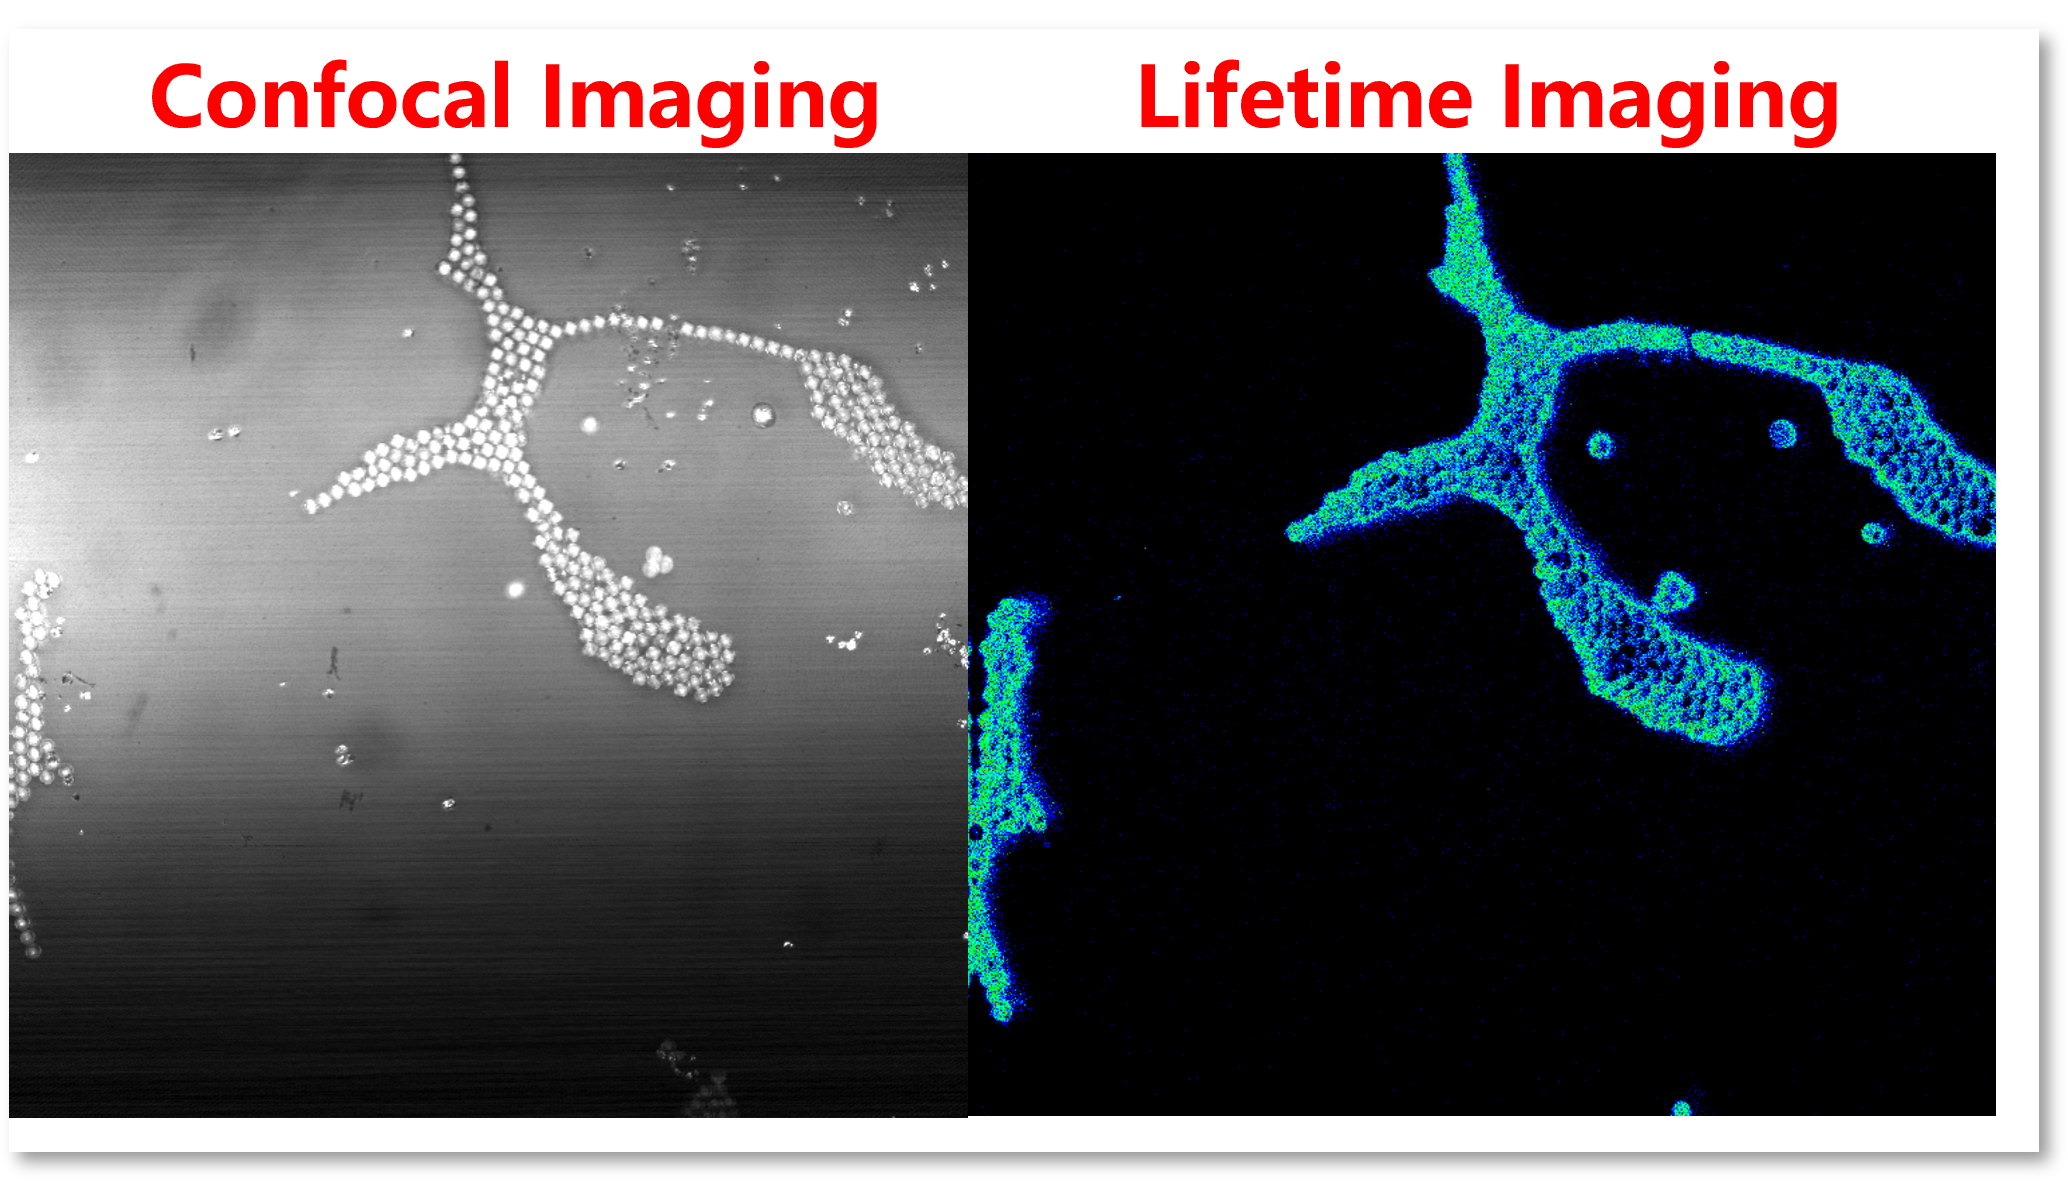
\includegraphics[width=\textwidth]{Fig/Fig21.png}
    \caption{}
    \label{fig21}
  \end{subfigure}

  \vspace{0.2cm}

  \begin{subfigure}[b]{0.7\textwidth}
    \centering
    \includegraphics[width=\textwidth]{Fig/Fig22.png}
    \caption{}
    \label{fig22}
  \end{subfigure}
  \bicaption{三路同步模式下的荧光寿命成像及与反射式图像、激发功率之间的关系。(a) 反射式共聚焦图像与三路同步 FLIM 图像对比；(b) 不同激发功率条件下的 TCSPC 成像结果}{FLIM results in the three-channel synchronized mode and their relationship to reflective imaging and excitation power. (a) Comparison between reflective confocal imaging and three-channel synchronized FLIM; (b) TCSPC imaging results obtained under different excitation-power conditions}
  \label{fig21-22}
\end{figure}



\section{FLIM 系统操作流程与数据处理链路}\label{5.4}

\begin{figure}[htbp]
  \centering
  \begin{subfigure}[b]{0.8\textwidth}
    \centering
    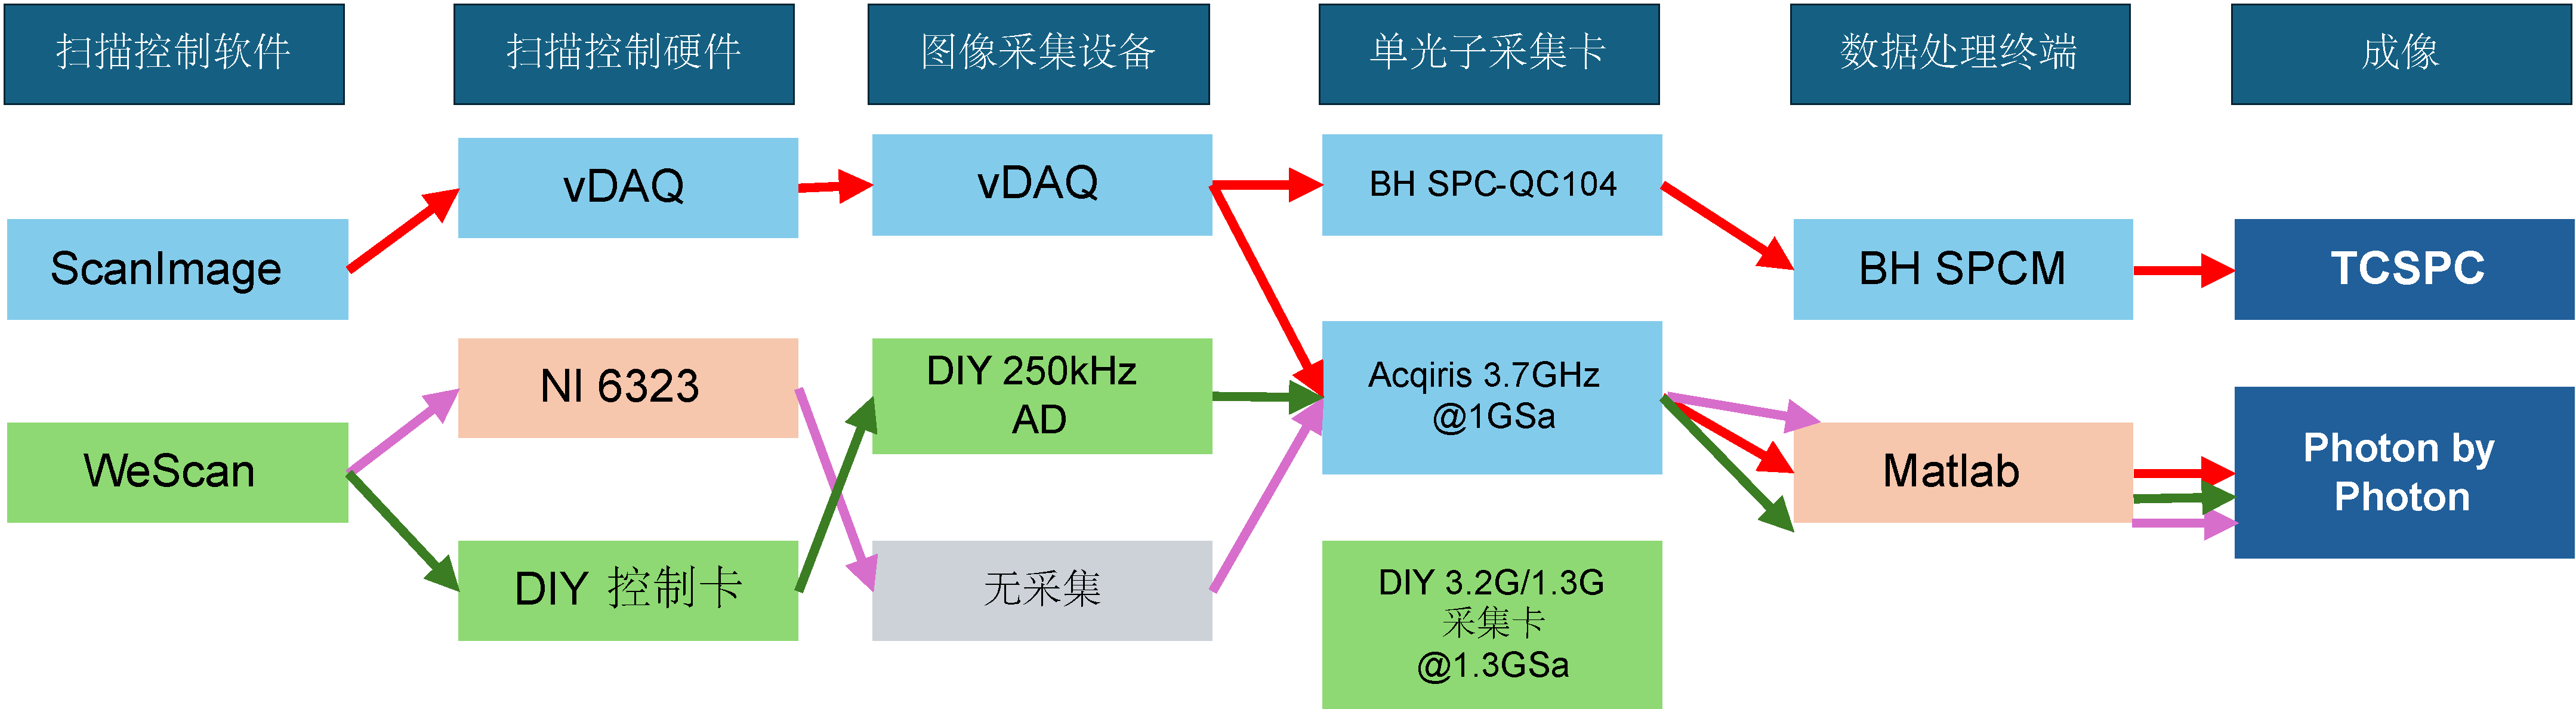
\includegraphics[width=\textwidth]{Fig/Fig24.pdf}
    \caption{}
    \label{fig24}
  \end{subfigure}
  \vspace{0.2cm}
  \begin{subfigure}[b]{0.8\textwidth}
    \centering
    \includegraphics[width=\textwidth]{Fig/Fig24.5.pdf}
    \caption{}
    \label{fig24.5}
  \end{subfigure}
  \bicaption{FLIM 数据处理链路与多路时序同步关系。(a) 当前已建立的荧光寿命成像处理流程；(b) 三路同步下 Frame、Line、Sync 及其合并信号的时序关系}{FLIM data-processing pipeline and multichannel synchronization timing. (a) Established fluorescence-lifetime imaging workflow; (b) timing relationship among the Frame, Line, Sync, and merged signals under three-channel synchronization}
  \label{fig24-24.5}
\end{figure}

在完成系统硬件搭建、IRF 标定和同步模式设计后，FLIM 实验还需要依赖明确的数据处理链路，才能将原始光子事件转化为可解释的寿命图像。结合本文所使用的硬件平台与控制方式，目前已建立三类互补的 FLIM 数据处理流程。

如图~\ref{fig24-24.5} 所示，本文目前建立的 FLIM 数据处理流程主要包括以下三类：

第一类为基于商用控制平台的三路同步 FLIM 流程。该流程利用商用 vDAQ 与 ScanImage 软件完成扫描控制与图像采集，并结合商用 TCSPC 板卡实现 pixel、line 和 frame 三路同步寿命成像。其优点是系统成熟、同步关系清晰、能够直接输出规则扫描区域下的寿命图像，适合标准 FLIM 实验和系统性能验证。

第二类为基于自研控制板卡的单路同步 FLIM 流程。该流程中，自研控制板卡的 DA 端口负责输出扫描与运动控制信号，AD 端口负责采集探测器输出，并结合 Acqiris 数据采集卡或自研 3.7\,GHz 采集卡完成单路同步寿命信息记录。该方式更适合灵活扫描、逐点分析和自定义数据处理，也为后续自研高速采集链路提供了平台基础。

第三类为基于单光子计数信号的逐像素重分配与拟合流程。该流程不依赖标准 TCSPC 图像文件的直接生成，而是先通过高速采集卡获取原始光子事件或脉冲响应，再结合扫描坐标信息完成逐像素重分配与寿命拟合。该方式虽然处理流程更复杂，但在硬件选择和算法实现上具有更高自由度，为非标准采集模式和后续算法优化提供了空间。

从实际操作流程看，这三类链路虽然实现方式不同，但基本步骤是一致的：首先完成扫描控制与同步触发，其次获取原始寿命相关数据，再结合同步信号进行空间重建，最后通过寿命拟合得到 FLIM 图像。图~\ref{fig24-24.5}(\subref{fig24.5}) 给出了三路同步模式下 frame、line、sync 以及合并触发信号之间的时序关系，说明了寿命采集并不是孤立的计时过程，而是与扫描系统严格耦合的时空映射过程。


\section{FLIM 成像结果与寿命拟合分析}\label{5.5}

在完成系统搭建、同步方式建立以及数据处理流程开发后，本文进一步对优化后的荧光寿命成像结果进行了实验验证。图~\ref{fig27} 给出了基于反射式参考成像、商用 TCSPC 采集以及单光子计数处理流程获得的 FLIM 对比结果。

图~\ref{fig27}(\subref{fig27a}) 为反射式共聚焦图像，用作样品空间分布的参考；图~\ref{fig27}(\subref{fig27b}) 为商用 TCSPC 板卡获得的荧光寿命图像，右侧色条表示不同像素对应的寿命值；图~\ref{fig27}(\subref{fig27c}) 表示在单路同步采集条件下，通过优化成像功率和采样参数后得到的信号分布；图~\ref{fig27}(\subref{fig27d}) 则是在此基础上进行逐像素寿命拟合后得到的寿命热图。

从结果上看，优化后的系统能够较清晰地恢复样品的空间轮廓及寿命分布信息。与原始测试结果相比，当前结果中局部过曝和光子堆积现象得到明显抑制，荧光微球边界更加清晰，寿命分布也更加稳定。说明通过对激发功率、采样参数及后续处理流程的联合优化，系统的寿命拟合质量和成像可靠性均得到了有效提升。

\begin{figure}[htbp]
    \centering
    \begin{subfigure}[b]{0.4\textwidth}
        \centering
        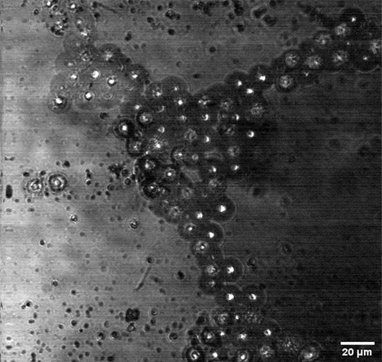
\includegraphics[width=\textwidth]{Fig/Fig27-1.png}
        \caption{}
        \label{fig27a}
    \end{subfigure}
    \hfil%
    \begin{subfigure}[b]{0.48\textwidth}
        \centering
        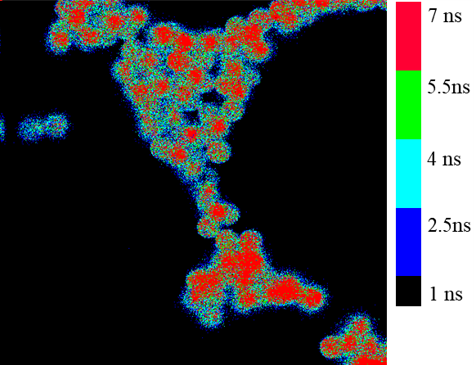
\includegraphics[width=\textwidth]{Fig/Fig27-2.png}
        \caption{}
        \label{fig27b}
    \end{subfigure}

    \vspace{0.25cm}

    \begin{subfigure}[b]{0.4\textwidth}
        \centering
        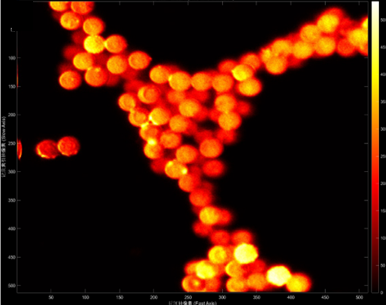
\includegraphics[width=\textwidth]{Fig/Fig27-3.png}
        \caption{}
        \label{fig27c}
    \end{subfigure}
    \hfil%
    \begin{subfigure}[b]{0.48\textwidth}
        \centering
        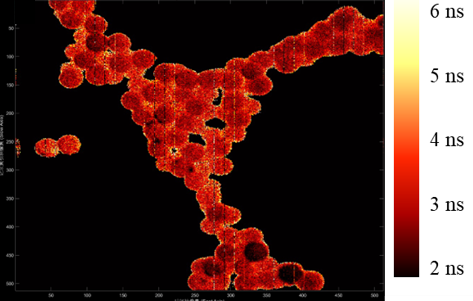
\includegraphics[width=\textwidth]{Fig/Fig27-4.png}
        \caption{}
        \label{fig27d}
    \end{subfigure}

    \bicaption{优化后的反射式、TCSPC 与单光子计数方式下的 FLIM 成像结果。(a) 反射式共聚焦参考图像；(b) 商用 TCSPC 板卡获得的荧光寿命图像；(c) 单路同步采集条件下优化后的信号分布；(d) 基于单光子计数流程重建得到的荧光寿命热图}
    {Optimized FLIM results obtained using reflective imaging, TCSPC, and the single-photon-counting workflow. (a) Reflective confocal reference image; (b) fluorescence-lifetime image acquired using a commercial TCSPC board; (c) optimized signal distribution under the single-channel synchronous acquisition mode; (d) fluorescence-lifetime heatmap reconstructed using the single-photon-counting workflow}
    \label{fig27}
\end{figure}


\begin{figure}[bhpt]
  \centering
  \begin{subfigure}[b]{0.25\textwidth}
    \centering
    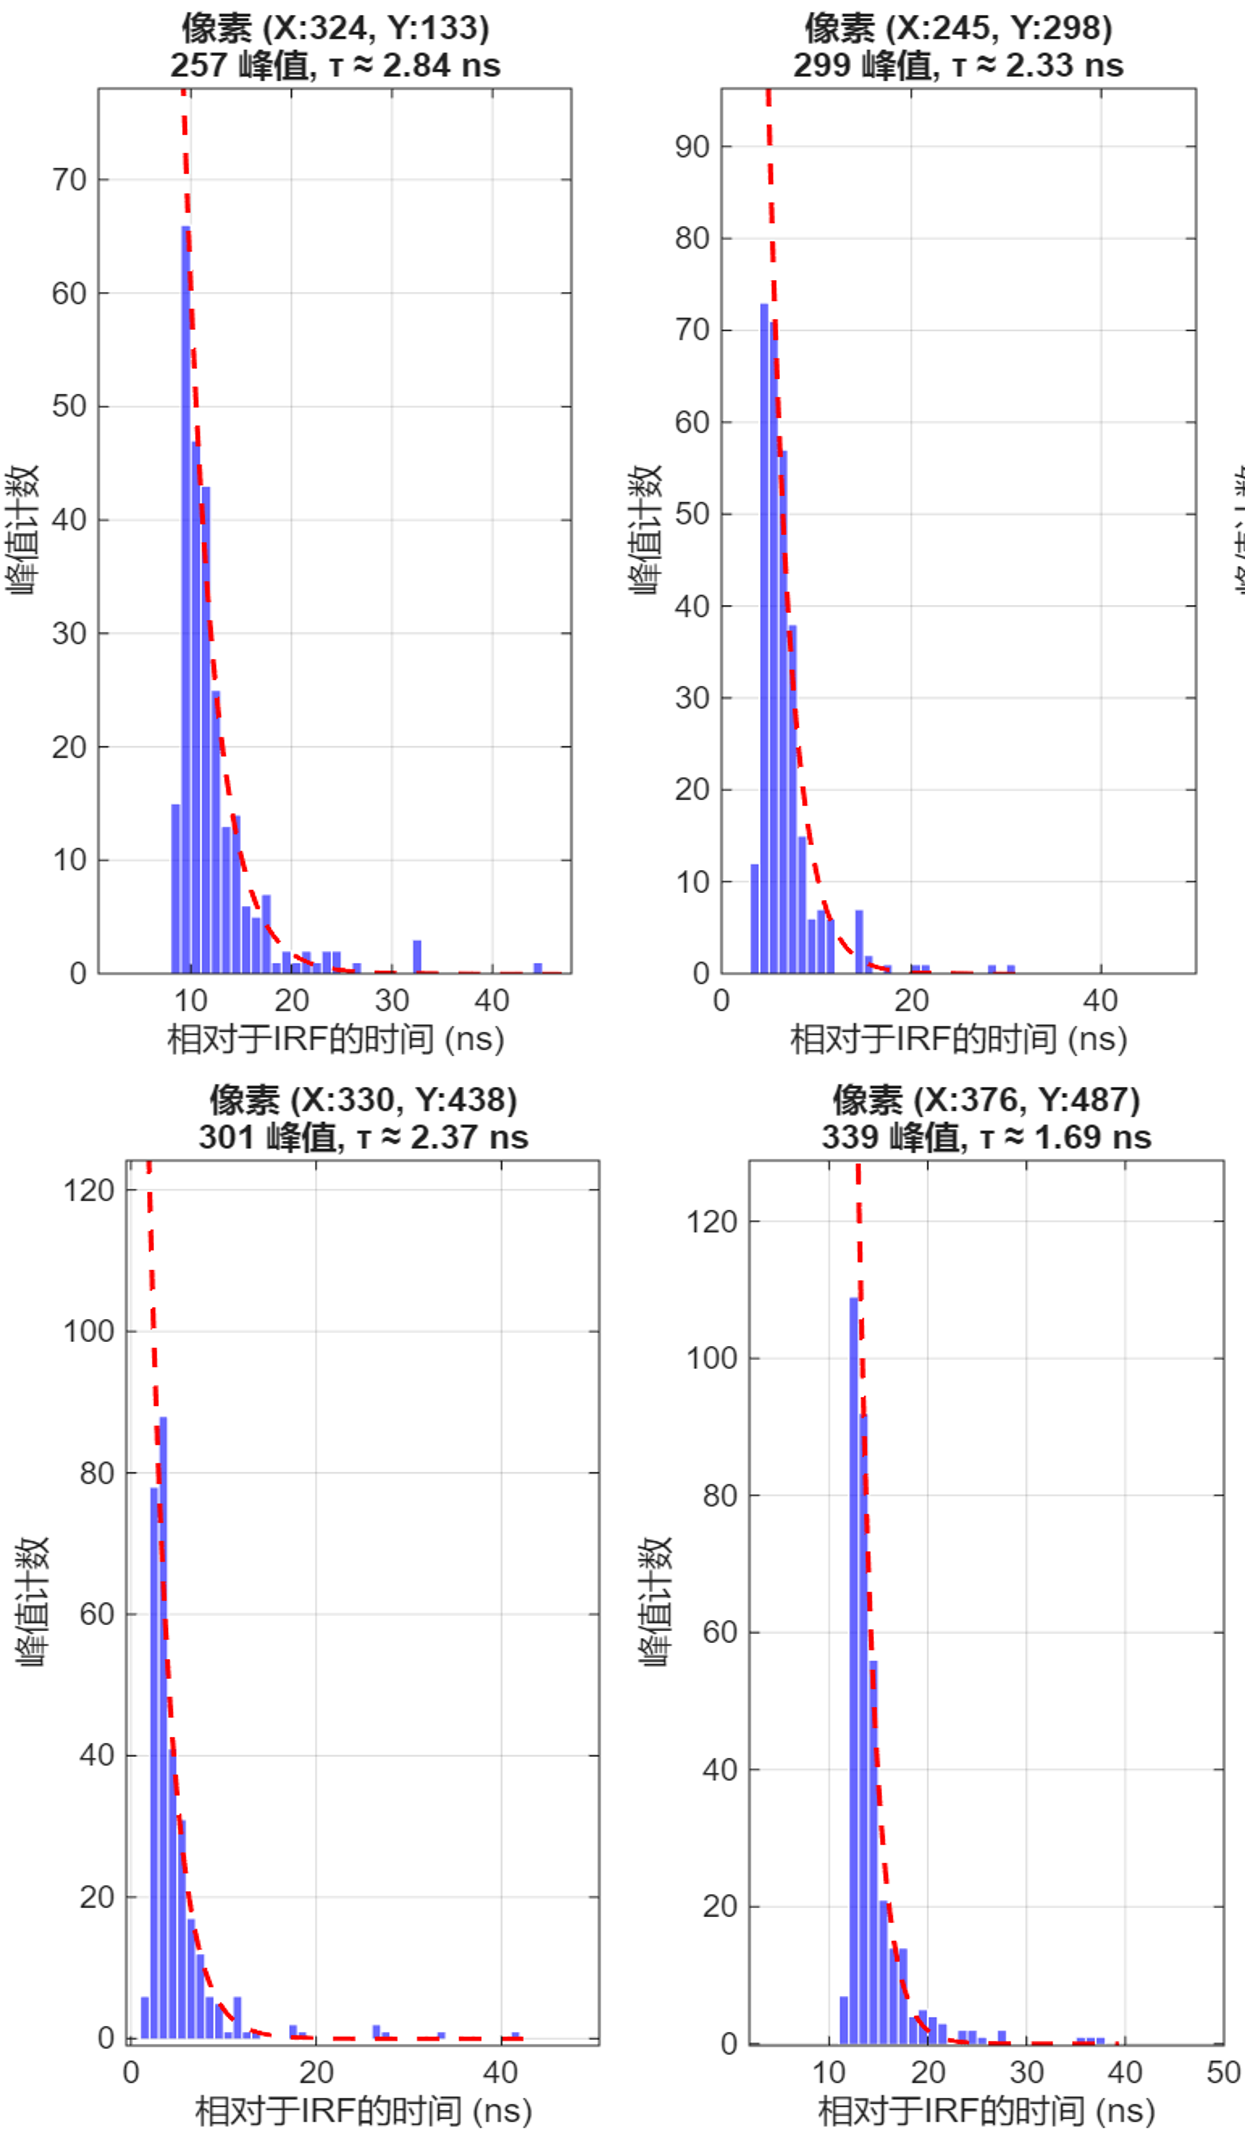
\includegraphics[width=\textwidth]{Fig/Fig28.png}
    \caption{}
    \label{fig28}
  \end{subfigure}
  \hfil
  \begin{subfigure}[b]{0.6\textwidth}
    \centering
    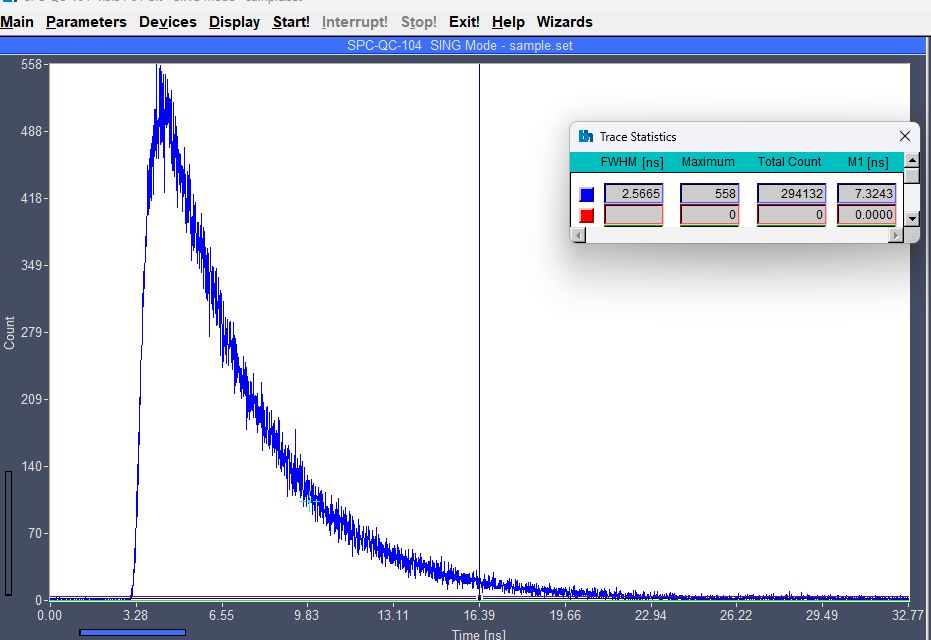
\includegraphics[width=\textwidth]{Fig/Fig28.6.png}
    \caption{}
    \label{Fig28.6}
  \end{subfigure}
  \bicaption{优化采集条件后的 FLIM 成像结果与逐像素寿命拟合分析。(a) 在单路同步荧光寿命模式下随机选取四个像素进行单指数拟合；(b) 对图a同样的条件下使用商用 SPCM 软件(Becker \& Hickl GmbH)拟合结果}{Optimized FLIM imaging results and pixel-wise lifetime-fitting analysis. (a) Randomly select four pixels for single exponential fitting in single channel synchronous fluorescence lifetime mode; (b) Fit the results using commercial SPCM software (Becker \& Hickl GmbH) under the same conditions as Figure a}
  \label{fig27-28}
\end{figure}


为了进一步验证逐像素寿命拟合结果的合理性，本文在图~\ref{fig27}(\subref{fig27d})中随机选取四个像素点，对其荧光衰减曲线进行单指数拟合，结果如图~\ref{fig28} 所示。拟合得到的寿命值主要分布在 1.6--2.4\,ns 范围内，说明系统能够稳定恢复纳秒量级的寿命信息。

作为对照，图~\ref{Fig28.6} 给出了商用 SPCM 软件获得的寿命拟合结果，其代表性寿命值约为 2.4\,ns。该结果与本文自建流程得到的拟合结果处于相同量级，并在主要寿命范围上具有较好一致性。由此说明，无论是基于商用 TCSPC 板卡的三路同步成像，还是基于单路同步与逐像素重分配的自研处理流程，均能够实现对荧光寿命的有效恢复。进一步地，这也验证了本文所构建 FLIM 系统及其数据处理链路在实验上具有可行性和可靠性。

图\ref{fig45}给出了在当前算法和单路同步采集模式下，利用 Acqiris 采集卡获得的荧光寿命分区结果。其中，图\ref{fig45}(\subref{fig45a})至图\ref{fig45}(\subref{fig45d})分别对应 $2\sim3$ ns、$3\sim4$ ns、$4\sim5$ ns 和 $>5$ ns 四个寿命区间。可以看出，样品的荧光寿命主要集中在 $2\sim4$ ns 范围内，其中 $2\sim3$ ns 和 $3\sim4$ ns 区间的像素分布最为密集，结构轮廓也最为完整，说明该范围内的寿命成分占主导地位，同时当前系统在该区间内具有较高的寿命解算精度与稳定性。相比之下，$4\sim5$ ns 及 $>5$ ns 区间的像素数量较少，分布相对稀疏，表明长寿命成分所占比例较低，且对应结果更易受到噪声影响。

\begin{figure}[bhpt]
    \centering
    \begin{subfigure}[b]{0.35\textwidth}
        \centering
        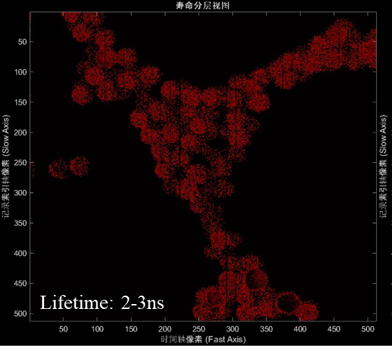
\includegraphics[width=\textwidth]{Fig/Fig45-1.png}
        \caption{}
        \label{fig45a}
    \end{subfigure}
    \hfil%
    \begin{subfigure}[b]{0.33\textwidth}
        \centering
        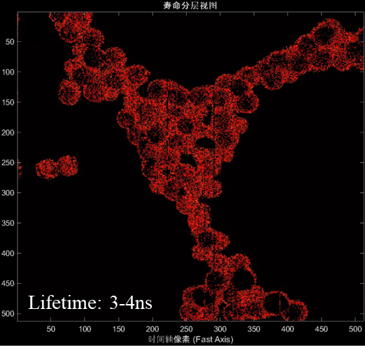
\includegraphics[width=\textwidth]{Fig/Fig45-2.png}
        \caption{}
        \label{fig45b}
    \end{subfigure}
    \vspace{0.2cm}
    \begin{subfigure}[b]{0.35\textwidth}
        \centering
        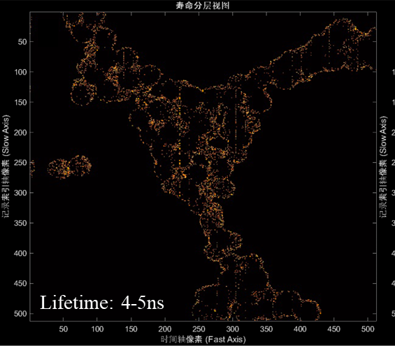
\includegraphics[width=\textwidth]{Fig/Fig45-3.png}
        \caption{}
        \label{fig45c}
    \end{subfigure}
    \hfil%
    \begin{subfigure}[b]{0.34\textwidth}
        \centering
        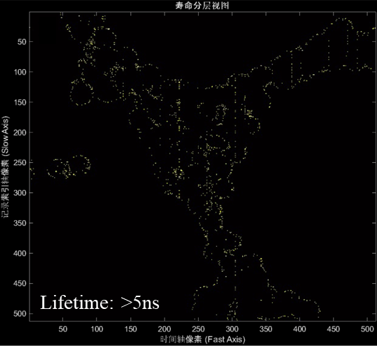
\includegraphics[width=\textwidth]{Fig/Fig45-4.png}
        \caption{}
        \label{fig45d}
    \end{subfigure}

    \bicaption{不同荧光寿命区间下样品轮廓与成分分布结果，展示了使用当前算法得到的荧光寿命切片能力。(a) $2\sim3$ ns；(b) $3\sim4$ ns；(c) $4\sim5$ ns；(d) $>5$ ns}
    {Lifetime-segmented images revealing sample contours and component distributions in different fluorescence-lifetime ranges. (a) $2\sim3$ ns; (b) $3\sim4$ ns; (c) $4\sim5$ ns; (d) $>5$ ns}
    \label{fig45}
\end{figure}


\section{硬件采集卡死区时间问题及优化}\label{5.6}

在单光子探测系统中，系统的总死区时间不仅受限于单光子雪崩二极管(SPAD)自身的物理特性，还受到数据采集卡(Data Acquisition, DAQ)硬件响应机制的制约。图~\ref{fig29} 从前端探测器响应、标准采集流程、采集卡重置限制以及长采集时间(long record)优化策略四个层面，给出了 SPAD 探测器与数据采集卡死区时间的时序分析示意。

其中，前两幅子图主要说明系统死区的来源与标准采集流程，后两幅子图则进一步展示采集卡在高计数率条件下的漏触发问题，及通过 long record 策略提升有效采集效率的实现思路。

如图~\ref{fig29}(\subref{fig29a}) 所示，当 SPAD 探测到光子并产生雪崩信号后，必须经历淬灭(quenching)与恢复(recovery)过程，才能重新进入可探测下一个光子的激活状态。这一段 SPAD 无法响应新光子的时间称为 SPAD 的物理死区时间，其典型值约为 50\,ns(以 Excelitas SPCM-AQRH-14 为例)。

除前端探测器的物理死区外，后端数据采集卡的信号处理流程同样会引入硬件死区。图~\ref{fig29}(\subref{fig29b}) 给出了标准采集窗口下采集卡对触发事件的记录过程；图~\ref{fig29}(\subref{fig29c}) 则进一步说明，在完成一次记录后，采集卡还需要经历数据读取和系统重置过程。经实际测量，Acqiris SA230P 采集卡的最小重置时间(rearm time)约为 23\,ns。当系统在高计数率下运行、相邻两次触发事件的间隔小于该重置时间时，采集卡将无法响应新的触发，从而导致有效光子事件丢失。

为了降低固定重置时间对系统整体探测效率的影响，本文采用了增加单次记录长度的优化策略，如图~\ref{fig29}(\subref{fig29d}) 所示。通过延长单次采集记录窗口，可以降低固定重置时间在总采集周期中的占比，从而提高系统的有效采集效率。系统的有效采集效率可定义为:

\begin{equation}
  \eta_{\mathrm{eff}} = \frac{T_{\mathrm{record}}}{T_{\mathrm{record}} + T_{\mathrm{rearm}}}
\end{equation}

其中，$T_{\mathrm{record}}$ 为单次记录时间，$T_{\mathrm{rearm}}$ 为固定硬件重置时间。由该式可见，在 $T_{\mathrm{rearm}}$ 固定的前提下，适当增大 $T_{\mathrm{record}}$ 可以显著提高有效记录时间在整个采集周期中的占比。

然而，记录长度也不能无限增加。过长的记录窗口会使单次传输数据量显著增大，若瞬时数据流超出硬件 FIFO 缓冲能力，或整体吞吐率超过计算机内存带宽、CPU 处理速度以及 SSD 持续写入能力，就可能引发缓存溢出、数据丢失甚至系统卡顿。因此，在实际系统配置中，必须在``提高有效采集效率''和``后端数据吞吐能力''之间进行折中，以获得最合适的记录长度设置。

综上，在 FLIM 系统中，探测效率不仅取决于 SPAD 本身的性能，还受到采集卡硬件死区与后端数据处理带宽的共同限制。通过合理设置单次记录长度、优化采集参数并控制计数率，可在保证数据完整性的前提下显著提高系统的有效采集能力。


\begin{figure}[htbp]
  \centering

  \begin{subfigure}[b]{0.80\textwidth}
    \centering
    \includegraphics[width=\textwidth]{Fig/Fig29-1.pdf}
    \caption{}
    \label{fig29a}
  \end{subfigure}

  \vspace{0.25cm}

  \begin{subfigure}[b]{0.34\textwidth}
    \centering
    \includegraphics[width=\textwidth]{Fig/Fig29-2.pdf}
    \caption{}
    \label{fig29b}
  \end{subfigure}\hfil%
  \begin{subfigure}[b]{0.42\textwidth}
    \centering
    \includegraphics[width=\textwidth]{Fig/Fig29-3.pdf}
    \caption{}
    \label{fig29c}
  \end{subfigure}

  \vspace{0.25cm}

  \begin{subfigure}[b]{0.80\textwidth}
    \centering
    \includegraphics[width=\textwidth]{Fig/Fig29-4.pdf}
    \caption{}
    \label{fig29d}
  \end{subfigure}

  \bicaption{SPAD 探测器与数据采集卡死区时间分析示意图。(a) SPAD 探测器的雪崩、淬灭与恢复过程及其物理死区时间；(b) 数据采集卡在标准采集窗口下对触发事件的记录流程；(c) 相邻触发间隔小于最小重置时间时采集卡的漏触发现象；(d) 采用 long record 策略降低固定重置时间占比、提升有效采集效率的示意图}
  {Schematic analysis of the dead times of the SPAD detector and data-acquisition card. (a) Avalanche, quenching and recovery process of the SPAD detector and its intrinsic dead time; (b) recording workflow of the data-acquisition card under the standard acquisition window; (c) missed-trigger effect when adjacent trigger intervals are shorter than the minimum rearm time; (d) schematic of improving effective acquisition efficiency by using the long-record strategy to reduce the fraction of fixed rearm time}
  \label{fig29}
\end{figure}


同时，根据图~\ref{fig19-20}(\subref{fig20})局部计数过高导致的死区问题，对于发光强度高的样品，会产生统计堆积，具体表现为图片过曝，需要降低功率或者增加扫描速度来降低局部计数率，避免死区时间过长导致的信号丢失和寿命拟合不准确等问题。因此针对荧光微球进行的荧光寿命实验中，激发功率的选择需要在保证足够信号强度的前提下，避免局部过曝和过高计数率引发的死区问题，从而获得稳定可靠的寿命拟合结果。根据图~\ref{fig45}的结果，其中子图\subref{fig45c}中可以看到，样品的边缘区域的寿命分布相对较长，且像素数量较少，这可能与边缘区域的信号较弱、计数率较低有关；而子图\subref{fig45a}和\subref{fig45b}中寿命分布较短、像素数量较多的区域，则可能对应样品的中心区域，信号较强、计数率较高。

这说明样品强度及死区时间效应可能会对荧光寿命拟合产生伪影，影响样品寿命信息判断，虽然对于荧光微球样品，在仔细调控激发功率后该结果仍在可接受范围内，但是仍然需要在后续实验中提高代码的鲁棒性，增加对死区效应的补偿机制，以进一步提升系统在高强度样品成像时的寿命拟合准确性和可靠性。例如可以通过对边缘信息进行识别，同时对拟合寿命进行补偿。

% \subsection{实验样品与成像条件}

% 本章系统验证采用荧光微球标准样品(江苏智川科技)。所用样品包括标称粒径 200 nm 和 10 μm 两类，其中 200 nm 荧光微球主要用于系统点扩散函数(point spread function, PSF)相关校正与成像链路检查，10 μm 荧光微球主要用于反射式参考成像、TCSPC 采集以及逐像素寿命拟合验证。采用尺寸远小于或接近系统分辨极限的荧光微球表征显微系统 PSF，是显微成像系统标定中的常用方法。

% 所用荧光微球的标称激发/发射峰包括 Ex\/Em = 450\/470 nm、488\/515 nm 和 532\/560 nm，其中以 488/515 nm 和 532\/560 nm 两种规格为主要实验样品；前者主要用于匹配 488 nm 皮秒激光激发以及 930 nm 多光子激发条件下的成像验证。样品平时于 4 \°C 条件下避光保存，成像前分散于 PBS 缓冲液中；实验过程中未对微球进行额外表面偶联或化学修饰。对于水相荧光微球，官方处理原则通常包括冷藏避光保存、使用前充分重悬，以及在出现团聚时通过涡旋或水浴超声实现重新分散。

% 本章 FLIM 实验的行扫描频率设为 213.5 Hz，图像分辨率为 515 $\times$ 512，帧频约为 0.417 Hz。激发功率和探测器增益根据样品亮度、局部计数率及图像动态范围进行联合调节，以在避免局部饱和和明显光子堆积的前提下获得稳定的寿命拟合结果。共聚焦实验采用 Mitutoyo M Plan Apo SL 20$\times$ 长工作距离无限远校正物镜(378-810-3，Mitutoyo)；该物镜产品页给出的标称工作距离为 30.5 mm，适用波段为 435--655 nm。多光子实验采用 Cousa 20$\times$ NA 0.5 空气物镜(Pacific Optica)；相关文献与厂商资料表明，该物镜为面向多光子成像优化的超长工作距离空气物镜，工作距离 20 mm，具有大视场特性。